\documentclass[11pt,a4paper]{article}
\usepackage{amsmath,amsfonts}
\usepackage{graphicx}
\usepackage{cite}
\usepackage{booktabs}
\usepackage[dvipsnames]{xcolor}
\usepackage{hyperref}
\usepackage[UTF8]{ctex}
\usepackage{float}
\usepackage{array}
\usepackage{multirow}
\usepackage{geometry}
\usepackage{setspace}
\usepackage{enumitem}
\usepackage{caption}
\usepackage{subcaption}
\usepackage{titlesec}
\usepackage{fancyhdr}
\usepackage{tabularx}
\usepackage{longtable}
\usepackage{balance}

\geometry{a4paper, left=2.5cm, right=2.5cm, top=2.8cm, bottom=2.5cm}
\onehalfspacing

\pagestyle{fancy}
\fancyhf{}
\fancyhead[L]{\small 探索性数据分析与可视化技术课程大作业}
\fancyhead[R]{\small 李盛鹏 · 2351136}
\fancyfoot[C]{\thepage}
\renewcommand{\headrulewidth}{0.4pt}

\hypersetup{
    colorlinks=true,
    linkcolor=blue!60!black,
    citecolor=blue!60!black,
    urlcolor=blue!60!black
}

\begin{document}

% ==================== 标题页 ====================
\begin{titlepage}
\centering
\vspace*{2cm}
{\LARGE\bfseries 基于 Zomato 数据的 Chennai 餐饮市场\\[0.4cm]
探索性数据分析与可视化研究}
\vspace{1.5cm}

{\large 《探索性数据分析与可视化技术》课程大作业报告}
\vspace{2cm}

{\large
\renewcommand{\arraystretch}{1.8}
\begin{tabular}{rl}
姓名：& {\bfseries 李盛鹏} \\
学号：& {\bfseries 2351136} \\
院系/班级：& {\bfseries 计算机科学与技术（数据科学与大数据技术）} \\
指导教师：& {\bfseries 王瀚漓} \\
提交日期：& \today
\end{tabular}
}

\vfill
{\small 本文为《探索性数据分析与可视化技术》课程期末大作业报告}
\end{titlepage}

% ==================== 摘要 ====================
\newpage
\thispagestyle{empty}
\begin{center}
{\Large\bfseries 摘\quad 要}
\end{center}
\vspace{0.5cm}

本报告围绕 Chennai 城市餐饮市场数据展开探索性数据分析与可视化研究。使用 Zomato 平台公开餐厅数据，从市场细分、空间分布、菜系与服务特征、品牌足迹以及评分预测等多个维度系统分析城市餐饮生态。项目首先对原始数据进行列名规范化、缺失值检查、多值文本拆分和衍生特征构造，然后结合统计分析、分布分析、空间分析和可视化设计方法，构建了多张面向洞察表达的图表，并在此基础上进一步引入机器学习预测模块，分析餐厅评分的关键驱动因素。

研究结果表明：Chennai 餐饮市场以 Dine-out 为主导，Cloud Kitchen 的平均评分最高；空间分布存在显著异质性，核心商圈与潜力区域在供给规模与评分水平上呈现差异；本地菜品和高频服务特征能够显著表征区域餐饮文化；品牌足迹、距城市中心距离和招牌菜丰富度是评分预测中的重要变量。该研究体现了探索性数据分析、数据预处理、信息可视化设计以及可视分析技术在真实课程项目中的综合运用。

\vspace{0.5cm}
\noindent\textbf{关键词：}探索性数据分析；可视化技术；餐饮数据；空间分析；市场细分；机器学习预测

% ==================== 目录 ====================
\newpage
\tableofcontents
\newpage

% ==================== 第一章 选题背景和意义 ====================
\section{选题背景和意义}

\subsection{行业背景与研究动机}

随着互联网技术和移动支付的快速发展，餐饮行业正加速向数字化方向转型。在线餐饮平台（如 Zomato、美团、大众点评等）的兴起，不仅改变了消费者的就餐决策方式，也为餐饮行业的数据化运营提供了丰富的数据基础~\cite{zomato}。餐厅信息、用户评分、菜品标签和服务特色等数据正在持续沉淀，形成了具有高维、多类型、多尺度特征的餐饮大数据。

对于消费者而言，平台数据能够辅助就餐决策——用户可以通过评分、菜品和服务特征快速筛选符合偏好的餐厅；对于商家和运营者而言，这类数据可以帮助理解市场竞争格局、识别潜在机会区域以及优化经营策略。例如，通过分析不同区域的餐厅供给密度和评分分布，可以发现竞争相对缓和但需求旺盛的蓝海市场；通过分析菜系和服务特征的组合模式，可以发现差异化经营的机会点。

Chennai（钦奈）作为印度第四大城市和重要的经济文化中心，具有以下特点使其成为理想的分析对象：
\begin{itemize}[leftmargin=2em]
    \item \textbf{人口密集、市场规模大}：Chennai 都市区人口超过 1,000 万，餐饮消费市场庞大且多元；
    \item \textbf{饮食文化多元}：兼具 South Indian、North Indian、Chinese、Continental 等多种菜系，本地特色菜品（如 Dosa、Idli、Filter Coffee、Biryani）具有鲜明的地域文化特征；
    \item \textbf{区域发展差异显著}：不同区域在经济发展水平、人口密度和消费能力上存在明显差异，为区域比较分析提供了天然条件；
    \item \textbf{数据可获得性好}：Zomato 平台在 Chennai 市场的覆盖率高，Kaggle 上有公开可用的数据集，便于开展分析研究。
\end{itemize}

本项目之所以选择 Chennai 餐饮市场作为探索性数据分析对象，主要基于三方面原因：
\begin{enumerate}[leftmargin=2em]
    \item 该主题具备明确的实际应用价值：消费者可借助分析结果比较不同区域、不同菜系和不同市场细分下的餐厅质量；餐饮从业者可借助分析判断区域供给密度、竞争压力和潜在选址机会；
    \item 该数据集包含评分、经纬度、区域、市场细分、服务特征、招牌菜和菜系等多种类型变量，适合综合运用课程中的统计分析、图形分析、空间可视化、文本标签展开和可视分析设计方法；
    \item 项目本身已实现了 Flask 驱动的交互式分析界面和多模块分析服务，具备从"数据处理"到"分析展示"再到"预测建模"的完整流程，适合作为课程大报告的研究载体。
\end{enumerate}

\subsection{研究意义}

本研究的意义主要体现在以下几个方面。

\begin{enumerate}[leftmargin=2em]
    \item \textbf{市场结构洞察意义}：通过分析 market segment、区域密度和评分分布，可以揭示 Chennai 餐饮市场的基本结构，帮助理解 Dine-out、Fast Food、Cloud Kitchen 等业态在规模与口碑上的差异。例如，Cloud Kitchen 作为近年来快速发展的餐饮模式，其评分表现是否优于传统 Dine-out 模式，是一个值得探究的问题。

    \item \textbf{空间分析意义}：通过区域聚合、密度分布和四象限矩阵，可以识别高供给高评分区、低供给高评分区、高供给低评分区和待发展区，为选址和区域竞争判断提供依据。这对于餐饮创业者选择开店位置、投资者评估区域潜力具有直接参考价值。

    \item \textbf{文化与消费行为意义}：通过菜系、菜品和服务特征分析，可以发现本地菜（如 Dosa、Idli、Filter Coffee）在覆盖率与口碑中的表现，体现数据背后的地方饮食文化特征。同时，通过热力图分析不同市场细分对服务特色的采用率，可以洞察不同业态经营模式的差异。

    \item \textbf{课程综合实践意义}：本项目将数据清洗、特征构造、统计描述、空间分析、可视化设计和机器学习预测有机整合，较完整地体现了探索性数据分析与可视化技术课程的核心知识点，是对课程理论知识的综合实践。
\end{enumerate}

\subsection{研究目标与方向}

结合课程要求和项目资源，本文将研究目标概括为以下四点：
\begin{enumerate}[leftmargin=2em]
    \item 从整体层面刻画 Chennai 餐饮市场的规模、评分分布和区域分布特征；
    \item 探究市场细分、区域、菜系、服务特色和招牌菜与评分之间的关系；
    \item 借助空间分析方法识别供给密度与质量水平之间的耦合或错位关系；
    \item 基于特征工程和机器学习模型，构建餐厅评分预测流程，并解释关键影响因素。
\end{enumerate}

% ==================== 第二章 相关方法 ====================
\section{相关方法}

\subsection{探索性数据分析方法}

探索性数据分析（Exploratory Data Analysis, EDA）由 John Tukey 于 1977 年提出~\cite{tukey}，强调在正式建模或推断之前，通过统计量、图形和交互分析理解数据结构、异常模式与变量关系。与验证性分析不同，EDA 更关注"发现问题"和"形成假设"，而非验证预先设定的假设。

EDA 的核心思想包括：
\begin{itemize}[leftmargin=2em]
    \item \textbf{抵抗性（Resistance）}：使用中位数、四分位数等稳健统计量，减少极端值对分析结论的影响；
    \item \textbf{残差分析（Residuals）}：通过观察残差分布判断模型假设是否成立；
    \item \textbf{重新表达（Re-expression）}：通过对数变换、标准化等手段改善数据的对称性和可比性；
    \item \textbf{图形化（Graphical Methods）}：利用图形的模式识别能力发现统计量难以捕捉的结构特征。
\end{itemize}

本研究中涉及的 EDA 方法主要包括：

\begin{enumerate}[leftmargin=2em]
    \item \textbf{描述性统计}：通过样本数、均值、中位数、标准差、最小值与最大值等指标快速把握数据整体分布。这是 EDA 的第一步，用于建立对数据全貌的基本认知；

    \item \textbf{分组聚合分析}：对 market segment、area、cuisine 等分类变量进行 groupby 聚合，比较不同类别在规模、评分和多样性上的差异。这种方法特别适合发现类别间的异质性；

    \item \textbf{分布分析}：利用直方图、脊线图和箱线图观察评分分布形态、离散程度及异常点情况。分布分析是理解核心变量特征的关键手段；

    \item \textbf{文本标签展开分析}：将 cuisine、features、top\_dishes 等逗号分隔文本拆分为长格式表，为高频项分析和交叉分析提供基础。这是处理多值文本字段的标准方法；

    \item \textbf{空间分析}：利用经纬度信息进行十六进制聚合、区域中心计算与四象限划分，识别空间异质性。空间 EDA 是地理数据特有的分析维度；

    \item \textbf{模型辅助分析}：利用回归模型、残差分解、Permutation Importance 和偏依赖分析（PDP）解释变量与评分之间的结构关系。这里将机器学习作为 EDA 的延展工具，而非单纯追求预测精度。
\end{enumerate}

上述方法之所以适用于本选题，是因为 Chennai 餐饮数据天然包含数值、类别、地理坐标和多值文本等多种数据类型，单一分析方法难以完整揭示其复杂性，必须通过多种 EDA 手段协同完成。

\subsection{数据可视化技术}

数据可视化的核心目标是将抽象数据映射为可理解的视觉编码~\cite{heer}，使分析结果更易被识别、比较和解释。William Cleveland 的图形感知理论指出，人类对位置编码的感知精度最高，其次是长度、角度、面积、颜色饱和度和颜色色相~\cite{cleveland}。这一理论指导了本项目中图表类型的选择。

本研究主要使用如下可视化技术：

\begin{enumerate}[leftmargin=2em]
    \item \textbf{统计图表}：包括柱状图（比较类别规模）、堆叠柱形图（展示结构组成）、直方图（展示分布形态）、箱线图（展示稳健分布特征）、热力图（展示二维关系矩阵）、气泡图（展示三变量关系）和六边形密度图（展示散点密集度）；

    \item \textbf{分布型图形}：使用脊线图（Ridgeline Plot）表现不同 market segment 的评分密度差异。脊线图通过将多条密度曲线垂直偏移排列，在同一坐标系中展示多组分布，特别适合比较多组数据的分布形态；

    \item \textbf{空间型图形}：借助经纬度生成空间热力分布和区域散布可视化。包括核密度估计（KDE）热力图、十六进制聚合密度图和地理散点图；

    \item \textbf{多维组合图}：在同一画布中同时展示"规模 + 平均评分""门店数 + 平均评分 + 链化程度"等信息，通过位置、大小和颜色的组合编码实现高维信息的低维表达；

    \item \textbf{文本可视化}：使用词云图（Word Cloud）展示区域名称的频率分布，直观呈现高频区域；

    \item \textbf{交互式前端可视化}：在项目实现中使用 Plotly、ECharts 和 Plotly Mapbox 支撑前端界面的探索式浏览，支持缩放、悬停提示和筛选等交互操作。
\end{enumerate}

这些技术的共同优势在于：既能支持定量比较，也能强化模式识别。例如，堆叠图适合展示不同区域评分等级构成，热力图适合展示 segment 与服务特征之间的采用率矩阵，六边形密度图适合观察预测值与真实值的一致性分布。

\subsection{可视分析技术与方法选择依据}

可视分析（Visual Analytics）强调"人机结合"的分析过程~\cite{ward}：先用算法提取结构，再通过可视化完成理解和解释。项目中的方法选择遵循以下依据：

\begin{enumerate}[leftmargin=2em]
    \item \textbf{变量类型匹配原则}：对于分类变量选用条形图、堆叠图或热力图；对于数值分布选用直方图、脊线图或箱线图；对于经纬度数据选用空间密度图和地理散点图。这一原则源于图形感知理论对不同编码方式感知效率的排序；

    \item \textbf{分析目标导向原则}：如果目标是比较规模，则选择条形图或排行榜；如果目标是观察评分形态，则选择分布图；如果目标是发现区域机会，则选择四象限矩阵。图表类型应服务于分析问题，而非反过来；

    \item \textbf{可读性与简洁性原则}：图中避免无效装饰（如 3D 效果、过多网格线），使用统一配色和清晰标签，并在必要时通过双色或渐变突出重点。Edward Tufte 提出的"数据-墨水比"（Data-Ink Ratio）原则~\cite{tufte}是这一原则的理论基础；

    \item \textbf{可解释性原则}：在机器学习部分优先选择便于解释的线性模型（Ridge、ElasticNet）与基于树的模型（RandomForest、HistGradientBoosting），再结合置换重要性和偏依赖图解释结果。模型可解释性是将预测结果转化为可行动洞察的关键。
\end{enumerate}

% ==================== 第三章 具体方法介绍 ====================
\section{具体方法介绍}

\subsection{数据来源与项目实现环境}

\subsubsection{数据来源}

本项目主要使用 Kaggle 数据集 \texttt{devvraj/chennai-restaurant-dataset}，数据来源于 Zomato 平台的 Chennai 餐厅公开信息。Zomato 是印度最大的在线餐饮平台之一，提供餐厅信息、用户评分、在线订餐和外卖配送等服务。该数据集通过 Zomato API 采集，涵盖了 Chennai 市区及周边地区的餐厅信息。

\subsubsection{系统实现环境}

系统实现上，项目采用 Flask 作为后端框架，遵循 Service -- Route -- Template 分层设计；分析脚本部分使用 Python 生态完成数据处理与图表生成；前端可视化模块则使用 Plotly、ECharts 和 JavaScript 进行页面渲染。具体技术栈如表~\ref{tab:techstack}所示。

\begin{table}[H]
\renewcommand{\arraystretch}{1.3}
\caption{项目技术栈}
\label{tab:techstack}
\centering
\begin{tabularx}{\textwidth}{lX}
\toprule
\textbf{层次} & \textbf{技术选型} \\
\midrule
后端框架 & Flask + Blueprint 路由模块，Service -- Route -- Template 分层设计 \\
数据处理 & Pandas（清洗/聚合）、NumPy（统计计算）、SciPy（核密度估计） \\
可视化 & Plotly.js（交互式图表）、ECharts（词云图）、Plotly Mapbox（地理空间可视化） \\
机器学习 & scikit-learn（Ridge / ElasticNet / RandomForest / HistGradientBoosting） \\
前端 & 原生 JavaScript、CSS 主题 \\
\bottomrule
\end{tabularx}
\end{table}

根据项目脚本与服务实现，分析工作流可分为"数据加载 $\rightarrow$ 数据预处理 $\rightarrow$ 长格式拆分 $\rightarrow$ 聚合分析 $\rightarrow$ 图表绘制 $\rightarrow$ 预测建模"六个阶段。

\subsection{数据预处理方法}

数据预处理是探索性数据分析的基础环节。高质量的分析结论必须建立在经过规范化处理的数据之上。本项目的数据预处理流程如表~\ref{tab:preprocessing}所示。

\begin{table}[H]
\renewcommand{\arraystretch}{1.3}
\caption{数据预处理流程概览}
\label{tab:preprocessing}
\centering
\begin{tabularx}{\textwidth}{clX}
\toprule
\textbf{步骤} & \textbf{操作} & \textbf{说明} \\
\midrule
1 & 数据完整性检查 & 检查缺失值、重复URL、数据类型一致性 \\
2 & 列名规范化 & 小写化、去特殊字符、下划线连接 \\
3 & 列验证与选择 & 仅保留11个核心分析字段 \\
4 & 衍生特征工程 & 新增评分分段、品牌足迹、空间偏移等特征 \\
5 & 多值文本展开 & 将逗号分隔文本拆分为长格式表 \\
\bottomrule
\end{tabularx}
\end{table}

\subsubsection{列名规范化与字段选择}

在脚本 \texttt{script/data\_processor.py} 中，首先调用 \texttt{normalize\_columns()} 对原始列名进行统一规范化，例如将 \texttt{Name\_of\_Restaurant} 映射为 \texttt{restaurant}、将 \texttt{Dining\_Rating} 映射为 \texttt{rating}、将 \texttt{Features/Category} 映射为 \texttt{features}。具体的列名映射关系如表~\ref{tab:column_mapping}所示。

\begin{table}[H]
\renewcommand{\arraystretch}{1.3}
\caption{列名规范化映射表}
\label{tab:column_mapping}
\centering
\begin{tabular}{lll}
\toprule
\textbf{原始列名} & \textbf{规范化后} & \textbf{处理方式} \\
\midrule
Name\_of\_Restaurant & restaurant & 小写，去特殊字符 \\
Dining\_Rating & rating & 小写，去特殊字符 \\
Area/Location & area & 小写，替换特殊字符 \\
Features/Category & features & 小写，替换特殊字符 \\
Market\_Segment & market\_segment & 小写，下划线连接 \\
Top\_Dishes & top\_dishes & 小写，下划线连接 \\
\bottomrule
\end{tabular}
\end{table}

随后依据 \texttt{EXPECTED\_COLUMNS} 仅保留 11 个核心字段：餐厅名称、服务特色、市场细分、菜系、招牌菜、地址、区域、经纬度、平台链接和评分。此步骤的主要作用是统一字段语义，为后续脚本处理和服务端分析提供稳定的数据模式。与课程中的数据清洗知识点对应，这一步属于"结构清洗"和"模式标准化"。

\subsubsection{完整性检查与缺失值处理}

数据完整性检查是预处理的第一步。主数据集 \texttt{Zomato\_Chennai\_Final.csv} 共 11,848 行、11 列，核心字段无缺失评分且无重复 URL，说明主表质量较高。作为对比，参考数据集 \texttt{Zomato\_Chennai\_Segmented.csv} 有 12,032 行但存在 3,274 个缺失值，这也解释了为何选择前者作为主分析数据集。

关键质量指标如表~\ref{tab:quality}所示。

\begin{table}[H]
\renewcommand{\arraystretch}{1.3}
\caption{主数据集关键质量指标}
\label{tab:quality}
\centering
\begin{tabular}{lc}
\toprule
\textbf{质量指标} & \textbf{数值} \\
\midrule
总餐厅数 & 11,848 \\
唯一餐厅名称数 & 8,352 \\
市场细分类型数 & 8 \\
覆盖区域数 & 268 \\
缺失评分数 & 0 \\
重复URL数 & 0 \\
评分均值 & 3.52 \\
评分中位数 & 3.6 \\
评分范围 & 0.3 -- 4.9 \\
纬度范围 & 12.6208 -- 13.1915 \\
经度范围 & 79.7042 -- 80.3001 \\
\bottomrule
\end{tabular}
\end{table}

脚本中对 \texttt{rating}、\texttt{latitude}、\texttt{longitude} 等字段通过 \texttt{pd.to\_numeric(errors="coerce")} 做类型转换，并在不同分析模块中通过 \texttt{dropna()} 去除无法参与计算的记录。由于主数据集评分字段完整，因此本研究未进行插值或模型填补，而是采用"删除不可用记录 + 保留高质量样本"的方式保证分析稳定性。

\subsubsection{特征构造}

项目在预处理阶段新增了多种衍生特征，以增强后续分析的深度和广度：

\begin{itemize}[leftmargin=2em]
    \item \textbf{唯一标识特征}：\texttt{restaurant\_id}，用于后续聚合与可视化追踪；

    \item \textbf{评分分段特征}：\texttt{rating\_band}，按以下阈值划分为五档：
    \begin{itemize}[leftmargin=1.5em]
        \item \texttt{fragile}：评分 $<$ 2.9
        \item \texttt{developing}：2.9 $\leq$ 评分 $<$ 3.4
        \item \texttt{solid}：3.4 $\leq$ 评分 $<$ 3.8
        \item \texttt{strong}：3.8 $\leq$ 评分 $<$ 4.2
        \item \texttt{elite}：评分 $\geq$ 4.2
    \end{itemize}

    \item \textbf{品牌足迹特征}：\texttt{same\_name\_outlets}（同名门店出现次数）和 \texttt{is\_multi\_outlet\_name}（是否为多门店品牌），通过餐厅名称出现频次衡量同名门店规模，用于分析品牌连锁效应；

    \item \textbf{文本统计特征}：在预测服务中，将 \texttt{cuisine}、\texttt{features}、\texttt{top\_dishes} 统一转为 token 串，并计算各自 token 数量，用于刻画菜系丰富度、服务多样性和菜品丰富度；

    \item \textbf{空间偏移特征}：以城市中位经纬度为基准，构造 \texttt{lat\_offset}、\texttt{lon\_offset} 和 \texttt{distance\_to\_city\_median\_km}，用于刻画餐厅相对城市中心的位置关系。
\end{itemize}

这些特征构造体现了课程中"从原始字段到分析变量"的思路，也为机器学习阶段提供了更具解释性的变量。

\subsubsection{多值文本展开}

数据中的 \texttt{cuisine}、\texttt{features} 和 \texttt{top\_dishes} 是逗号分隔的多值文本字段。例如，一条餐厅记录的 cuisine 字段可能为"Biryani, North Indian, Mughlai, Desserts"。为了支持按标签统计和交叉分析，项目通过 \texttt{explode\_attribute()} 函数将这些字段拆分为三张长格式表。具体的展开统计如表~\ref{tab:longformat}所示。

\begin{table}[H]
\renewcommand{\arraystretch}{1.3}
\caption{多值文本展开统计}
\label{tab:longformat}
\centering
\begin{tabular}{lcccc}
\toprule
\textbf{维度} & \textbf{原始行数} & \textbf{长格式行数} & \textbf{唯一值数} & \textbf{膨胀倍数} \\
\midrule
菜系（cuisine） & 11,848 & 28,799 & 92 & 2.43$\times$ \\
特色（features） & 11,848 & 32,698 & 78 & 2.76$\times$ \\
菜品（top\_dishes） & 11,848 & 76,763 & 2,036 & 6.48$\times$ \\
\bottomrule
\end{tabular}
\end{table}

这一过程本质上属于数据变换与重塑（reshape），是将"宽表中的多值文本"转为"适合分组统计的长表"，也是后续热力图、菜系排行和菜品分析的基础。展开后的长格式表保留了 \texttt{restaurant\_id}、\texttt{market\_segment}、\texttt{area}、\texttt{rating} 等基础列，确保可以与原始表进行关联分析。

\subsection{探索性分析方法}

\subsubsection{描述性统计与分组聚合}

项目使用 Pandas \texttt{groupby()} 和聚合函数计算整体指标与分组指标，包括：
\begin{itemize}[leftmargin=2em]
    \item 样本总数、区域数、细分市场数、均值、中位数、标准差等全局统计量；
    \item 各市场细分的门店数、平均评分、中位数和链化占比；
    \item 各区域的门店数、平均评分、经纬度中心和细分多样性；
    \item 各菜系、菜品和服务特征的出现频次和平均评分。
\end{itemize}

这类方法适用于建立"数据全貌"和"类别差异"认知，是典型的 EDA 起点。

\subsubsection{分布分析}

项目针对评分这一核心变量使用了多种分布分析图形：
\begin{itemize}[leftmargin=2em]
    \item \textbf{直方图}：展示整体评分和分组评分的频数分布，bin 宽度设为 0.3，适合观察分布的集中趋势和偏态；

    \item \textbf{脊线图}：对不同 market segment 的评分密度曲线进行横向比较。脊线图通过将多条核密度估计曲线垂直偏移排列，可以直观展示"谁更集中、谁更偏高、谁波动更大"；

    \item \textbf{箱线图}：识别不同区域评分的中位数、四分位间距和异常值。箱线图的优势在于能够同时展示中心趋势、离散程度和异常值三个维度；

    \item \textbf{堆叠柱形图}：比较不同区域在五档 rating\_band 下的结构差异，展示各区域评分等级的构成比例。
\end{itemize}

\subsubsection{空间分析}

空间分析部分主要基于经纬度和区域聚合结果展开，包括：
\begin{itemize}[leftmargin=2em]
    \item 对门店位置进行十六进制聚合，生成餐厅密度热力图，揭示餐厅供给的空间聚集模式；
    \item 对平均评分进行空间聚合，观察评分表面的变化趋势；
    \item 按区域计算餐厅供给量与平均评分，并结合中位值构造四象限矩阵（详见图~\ref{fig:quadrant}）；
    \item 基于区域统计构建气泡图，以餐厅数、平均评分和区域规模三维度观察区域差异；
    \item 使用核密度估计（KDE）生成空间热力分布，观察餐厅分布的"沿海密集、内陆疏松"格局。
\end{itemize}

在 \texttt{app/services/spatial\_service.py} 中，四象限分析以区域餐厅数中位数和平均评分中位数作为阈值，将区域划分为四类：
\begin{itemize}[leftmargin=2em]
    \item \textbf{Mature \& Quality}（高供给、高评分）：成熟优质餐饮区；
    \item \textbf{Hidden Gem / Potential}（低供给、高评分）：小而美/潜力区；
    \item \textbf{Competitive \& Volatile}（高供给、低评分）：竞争激烈但质量不稳定区；
    \item \textbf{Underdeveloped}（低供给、低评分）：待发展区。
\end{itemize}

\subsubsection{机器学习辅助分析}

除了传统 EDA，本项目还将探索性分析延伸至"预测 + 可解释分析"。机器学习在这里不是作为最终目标，而是作为 EDA 的延展工具，用来回答"评分由哪些因素驱动""哪些细分或区域更难预测"等更深层问题。

具体方法包括：
\begin{itemize}[leftmargin=2em]
    \item 使用 \texttt{GroupShuffleSplit} 按餐厅名分组划分训练集与测试集，避免同名门店在训练和测试之间泄漏信息；
    \item 构建多种回归模型进行对比：
    \begin{itemize}[leftmargin=1.5em]
        \item DummyRegressor（基线模型，使用均值或中位数预测）
        \item Ridge 回归（L2 正则化线性模型）
        \item ElasticNet 回归（L1+L2 混合正则化线性模型）
        \item RandomForest 回归器（基于 Bagging 的集成模型）
        \item HistGradientBoosting 回归器（基于 Boosting 的高效梯度提升模型）
    \end{itemize}
    \item 使用 MAE（平均绝对误差）、RMSE（均方根误差）与 $R^2$（决定系数）评价模型性能；
    \item 对最佳模型进行残差分析、误差分组分解、Permutation Importance（置换重要性）和偏依赖分析（PDP）。
\end{itemize}

特征工程方面，对分类变量（market\_segment、area）进行 One-Hot 编码，对数值变量进行中位数填补与标准化，对菜系、服务和招牌菜 token 分别使用 CountVectorizer 和 TF-IDF 向量化。

\subsection{可视化设计与实现方法}

本项目在图表设计中遵循了四项核心原则：

\begin{enumerate}[leftmargin=2em]
    \item \textbf{准确性}：根据变量类型选择合适图表，避免使用误导性 3D 图、面积图或不恰当比例。例如，评分分布使用直方图而非饼图，区域比较使用柱状图而非雷达图；

    \item \textbf{清晰性}：通过统一调色板、标题、副标题、标注和图例增强图形可读性。每个图表都包含明确的标题、轴标签和必要的注释；

    \item \textbf{简洁性}：在 \texttt{visualizations.py} 中统一使用 \texttt{clean\_axis()}、\texttt{add\_panel\_title()} 等辅助函数减少视觉冗余，去除不必要的网格线和边框；

    \item \textbf{一致性}：采用暖色美食主题配色（Indian food-inspired color palette），将图形风格、字体和标题结构保持一致，增强多图联读能力。统一的配色方案确保不同图表之间具有视觉连贯性。
\end{enumerate}

从实现方式上看，离线图表主要使用 Matplotlib 生成 PNG；在线交互界面则由 Plotly、ECharts 和 JavaScript 负责渲染。这样的双路线实现既满足了课程纸质报告的静态插图需求，也保留了系统层面的交互能力。

% ==================== 第四章 分析展示 ====================
\section{分析展示}

\subsection{数据概况与整体结构}

数据集主表共包含 11,848 家餐厅记录，覆盖 268 个区域和 8 类市场细分，平均评分为 3.52，中位数为 3.6，说明整体评分分布偏向中高分区域，但波动性仍然存在。多值文本展开后，菜系标签达到 92 种，服务特色达到 78 种，菜品标签达到 2,036 种，充分说明该数据集具有较高的多样性和分析价值。

\begin{figure}[H]
\centering
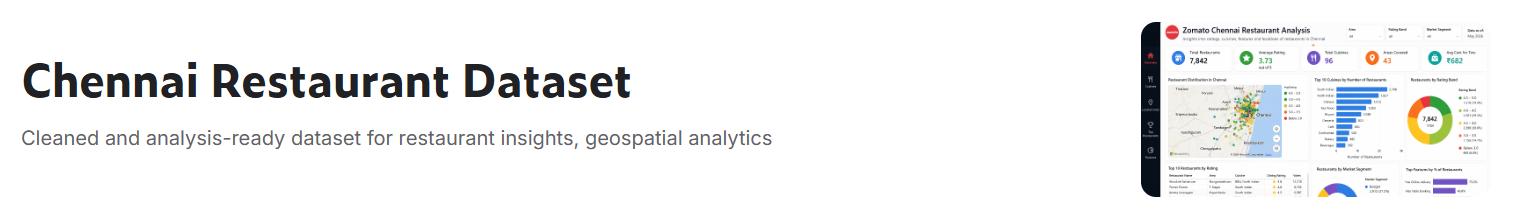
\includegraphics[width=0.95\textwidth]{figures/30_dataset_screenshot.png}
\caption{主数据集原始字段预览}
\label{fig:dataset_screenshot}
\end{figure}

图~\ref{fig:dataset_screenshot} 展示了原始数据集的字段结构，可以看到数据包含餐厅名称、评分、菜系、市场细分、服务特色、招牌菜、地址、区域和地理坐标等核心字段。

\begin{figure}[H]
\centering
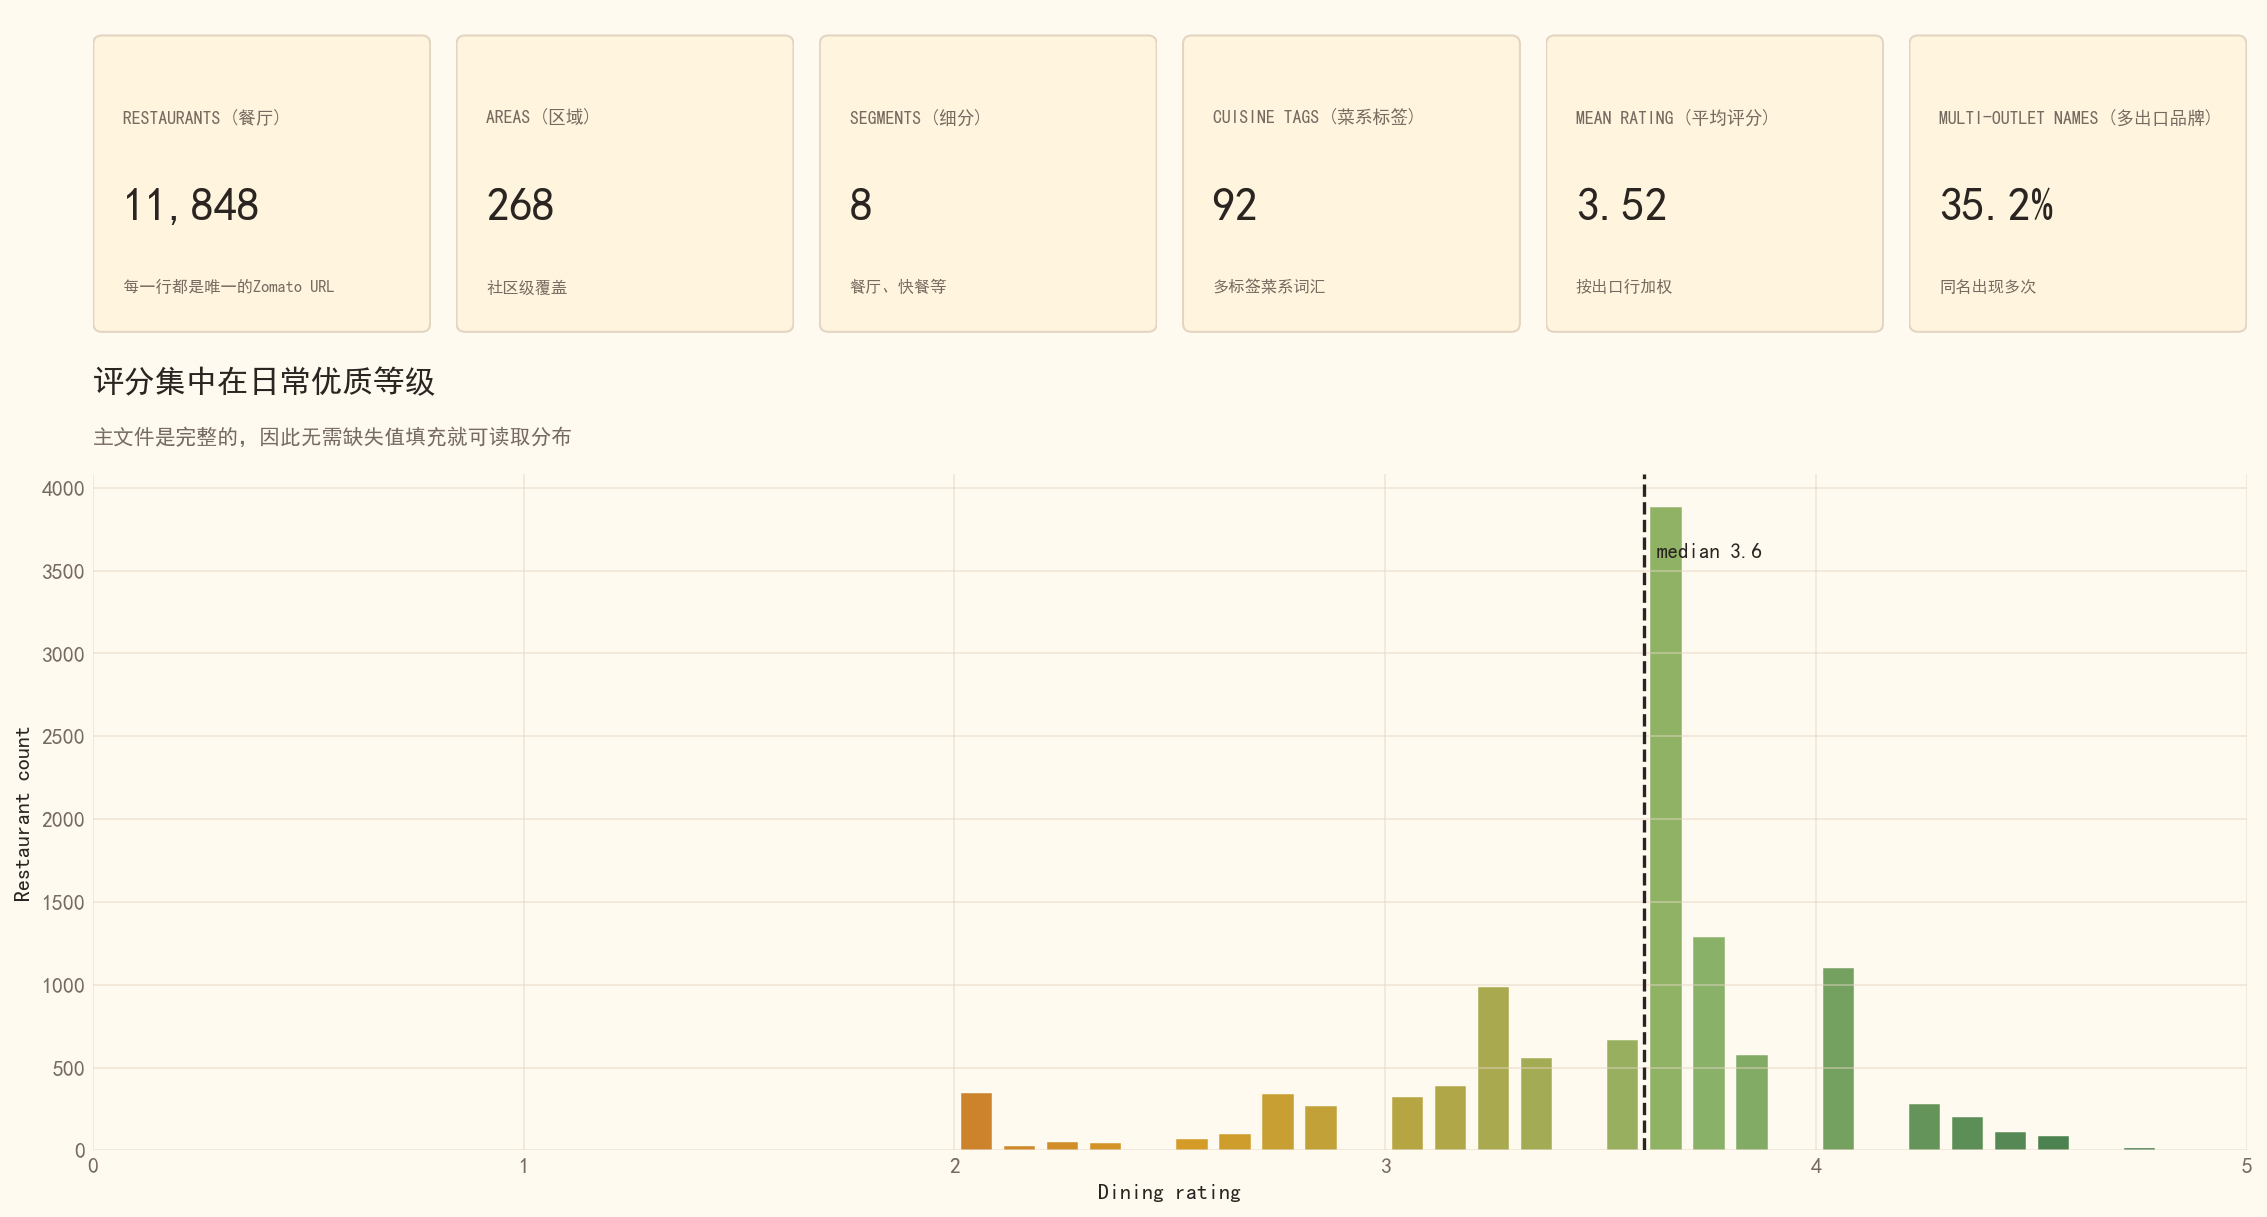
\includegraphics[width=0.95\textwidth]{figures/01_scorecard.png}
\caption{数据概况评分卡与整体评分分布}
\label{fig:scorecard}
\end{figure}

图~\ref{fig:scorecard} 展示了数据规模、区域覆盖、细分市场数量、菜系标签规模以及整体评分分布。评分直方图显示大多数餐厅集中在 3.0--4.0 分区间，结合中位数 3.6 可以推断平台评分存在一定"高分聚集"现象，因此分析时更应重视相对差异而非绝对高低。

\subsection{市场细分与评分差异分析}

市场细分分析表明，Chennai 餐饮市场以 Dine-out 为主导，门店数达到 5,292；第二梯队包括 Delivery / Fast Food 等高频业态；Cloud Kitchen 虽然规模并非最大，但平均评分达到 3.68，是所有细分市场中表现最优的类型之一。这说明"高供给"和"高评分"并不是同一维度的问题。

\begin{figure}[H]
\centering
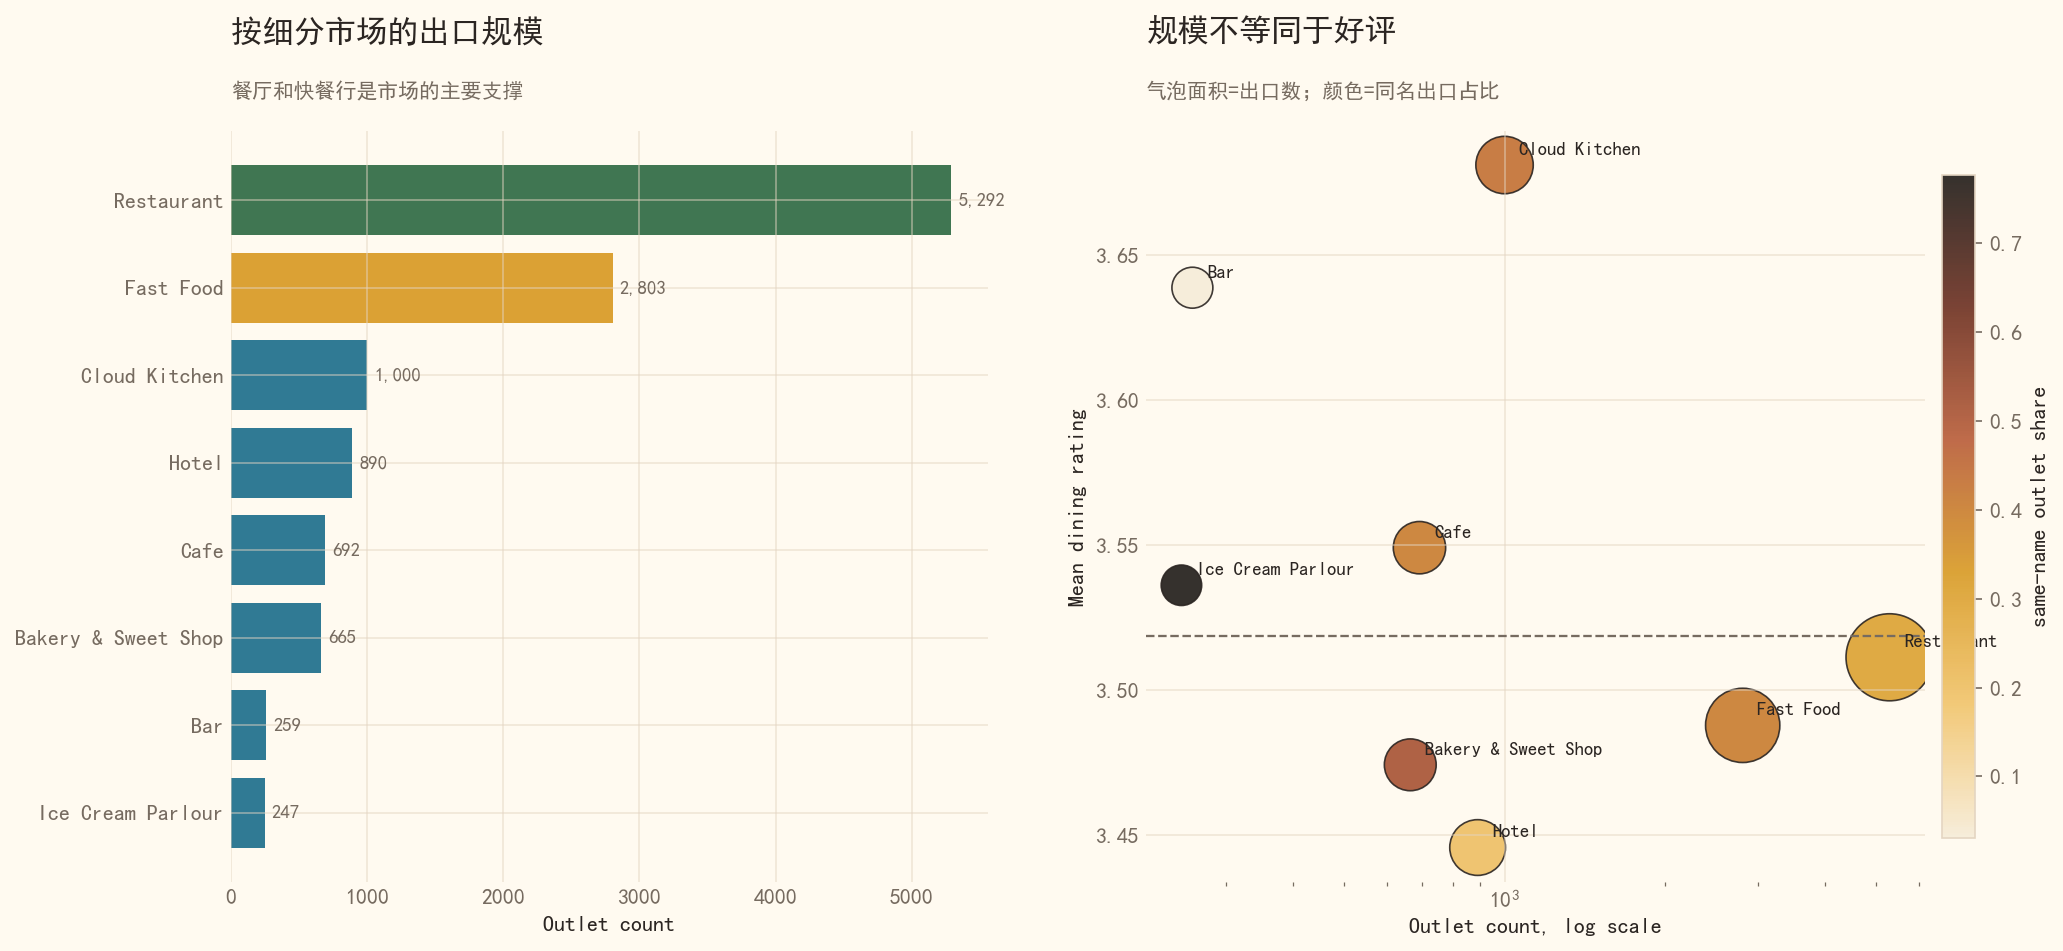
\includegraphics[width=0.95\textwidth]{figures/02_segment_analysis.png}
\caption{市场细分规模、评分与链化程度分析}
\label{fig:segment}
\end{figure}

图~\ref{fig:segment} 左侧条形图体现了不同细分市场的供给规模，右侧气泡图则联合展示了平均评分、门店数和同名门店占比。从图中可以观察到，Dine-out 在门店数量上占据绝对优势，而 Cloud Kitchen 和 Dessert Parlours 在评分上表现较好。

\begin{figure}[H]
\centering
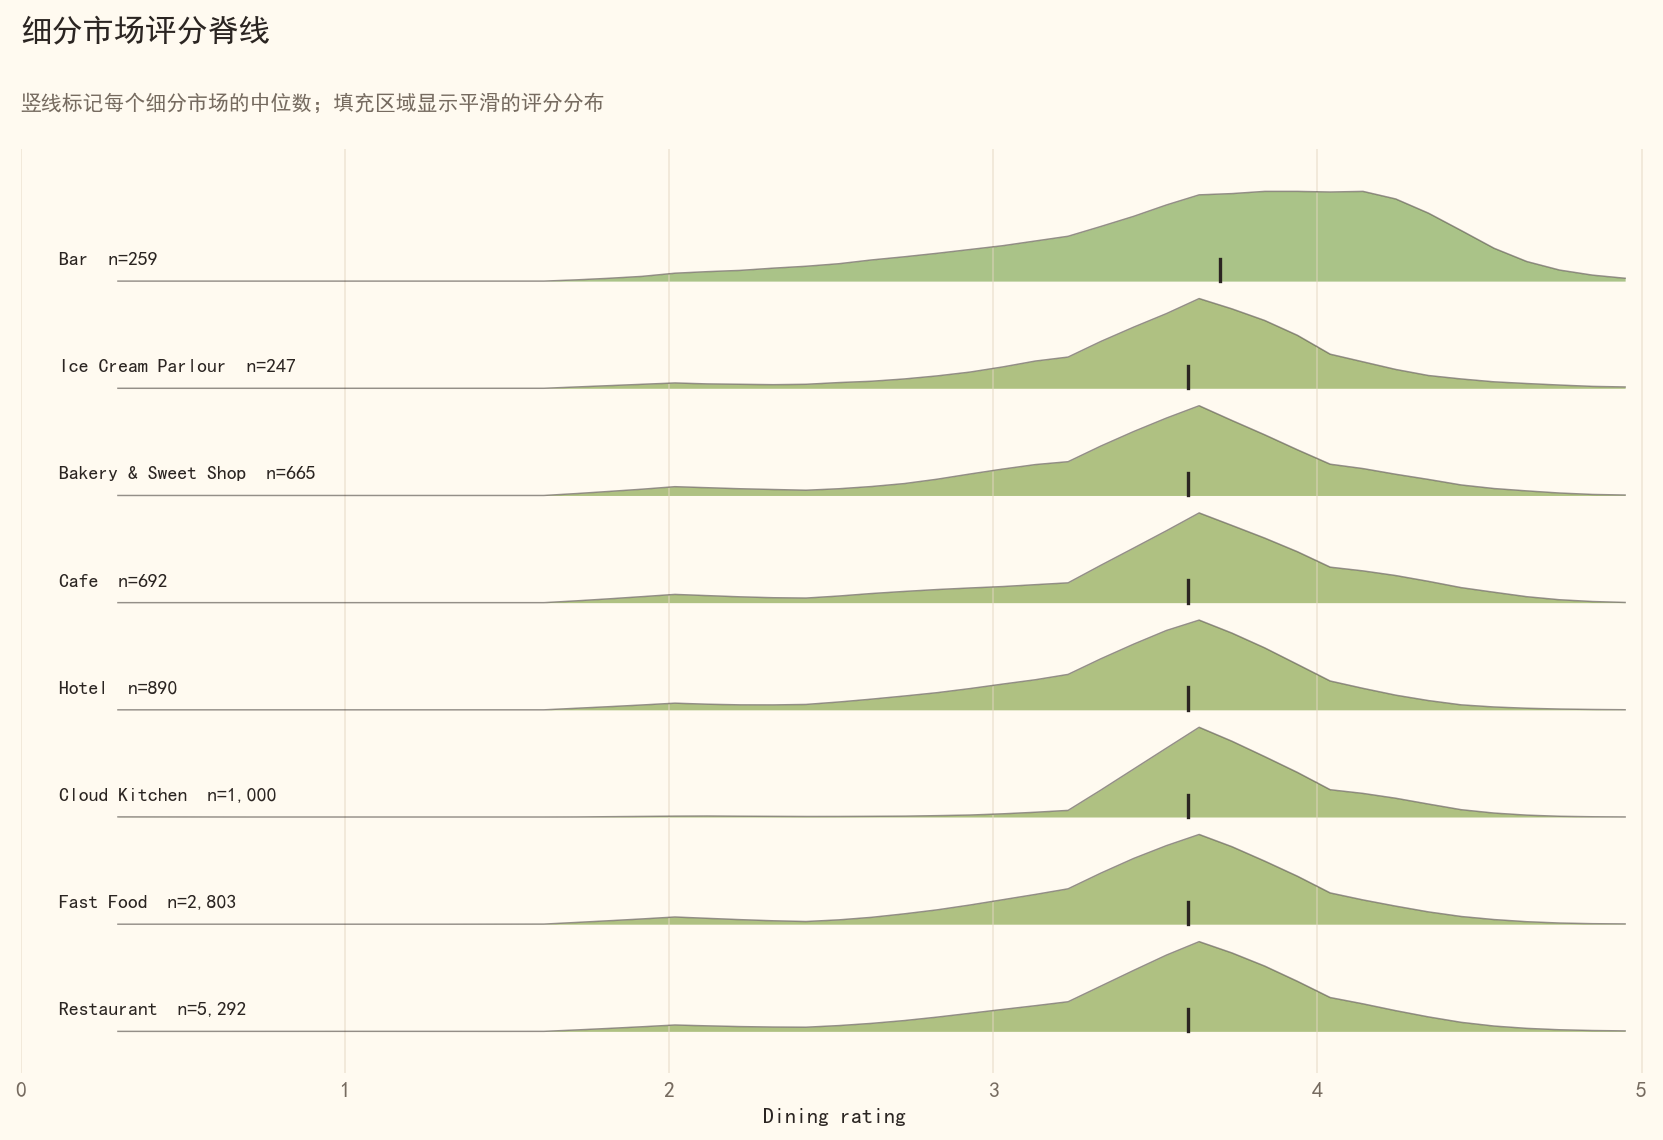
\includegraphics[width=0.95\textwidth]{figures/03_rating_ridgelines.png}
\caption{不同市场细分的评分脊线分布}
\label{fig:ridgeline}
\end{figure}

图~\ref{fig:ridgeline} 进一步表明：不同细分市场的评分分布形态并不一致，部分细分市场虽然平均评分相近，但分布宽度和中位数存在明显差异。这种差异说明仅看均值容易掩盖结构问题，分布型图形在 EDA 中具有不可替代的作用。

\subsection{EDA 交互界面分析}

除静态图表外，项目还实现了基于 Flask 的交互式 EDA 界面，支持更灵活的数据探索。

\begin{figure}[H]
\centering
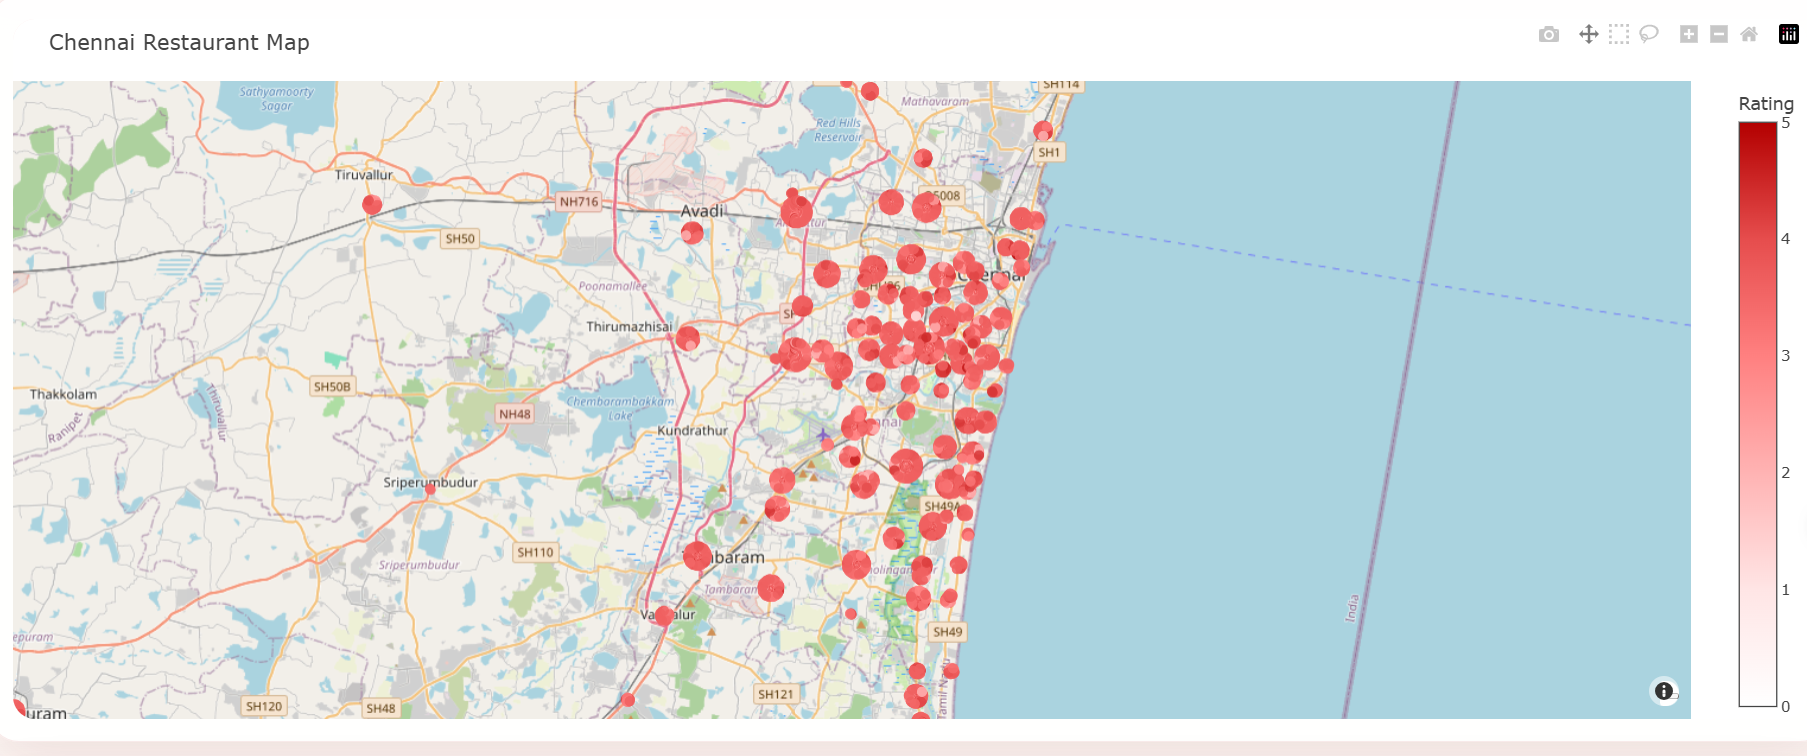
\includegraphics[width=0.95\textwidth]{figures/09_overview_scatter_map.png}
\caption{EDA 交互界面概览：散点地图与评分分布}
\label{fig:overview_eda}
\end{figure}

图~\ref{fig:overview_eda} 展示了 EDA 交互界面的概览页面，包含基于 Plotly Mapbox 的 Chennai 全市餐厅空间散点地图（颜色编码评分高低）和评分分布直方图。用户可以通过缩放、平移和悬停查看单个餐厅的详细信息。

\begin{figure}[H]
\centering
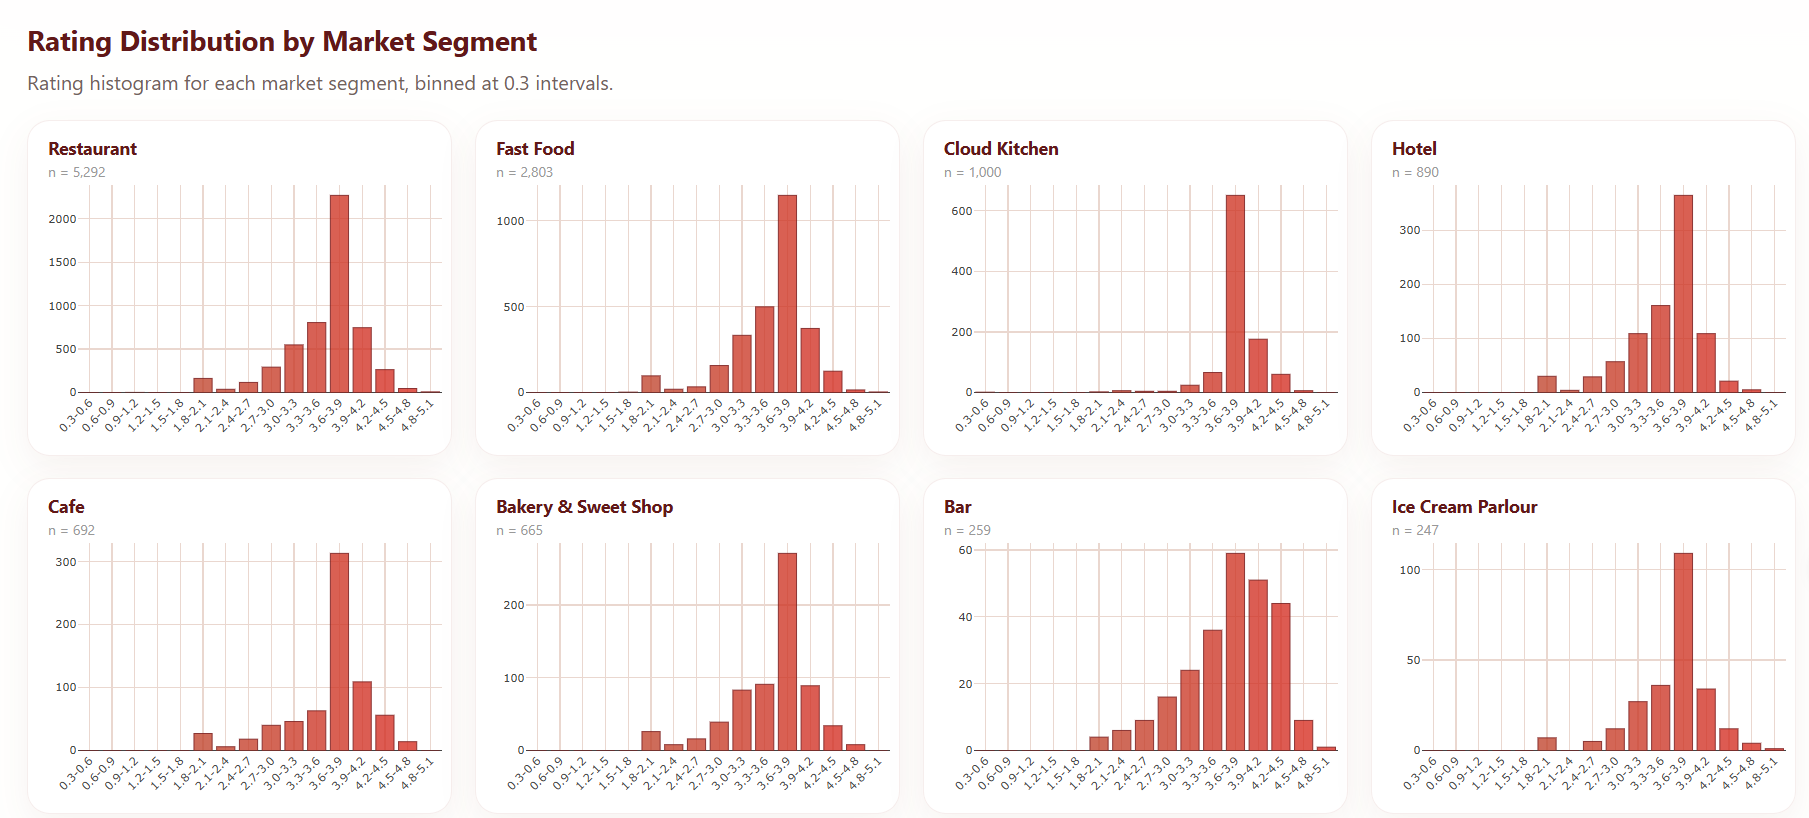
\includegraphics[width=0.95\textwidth]{figures/10_market_segment_histogram.png}
\caption{Market Segment 评分直方图}
\label{fig:segment_histogram}
\end{figure}

图~\ref{fig:segment_histogram} 以分面直方图的形式展示了 8 种市场细分的评分分布。bin 宽度设为 0.3，可以观察到不同细分市场的评分分布形态存在差异：部分细分市场的评分分布较为集中，而另一些则呈现较宽的分布。

\begin{figure}[H]
\centering
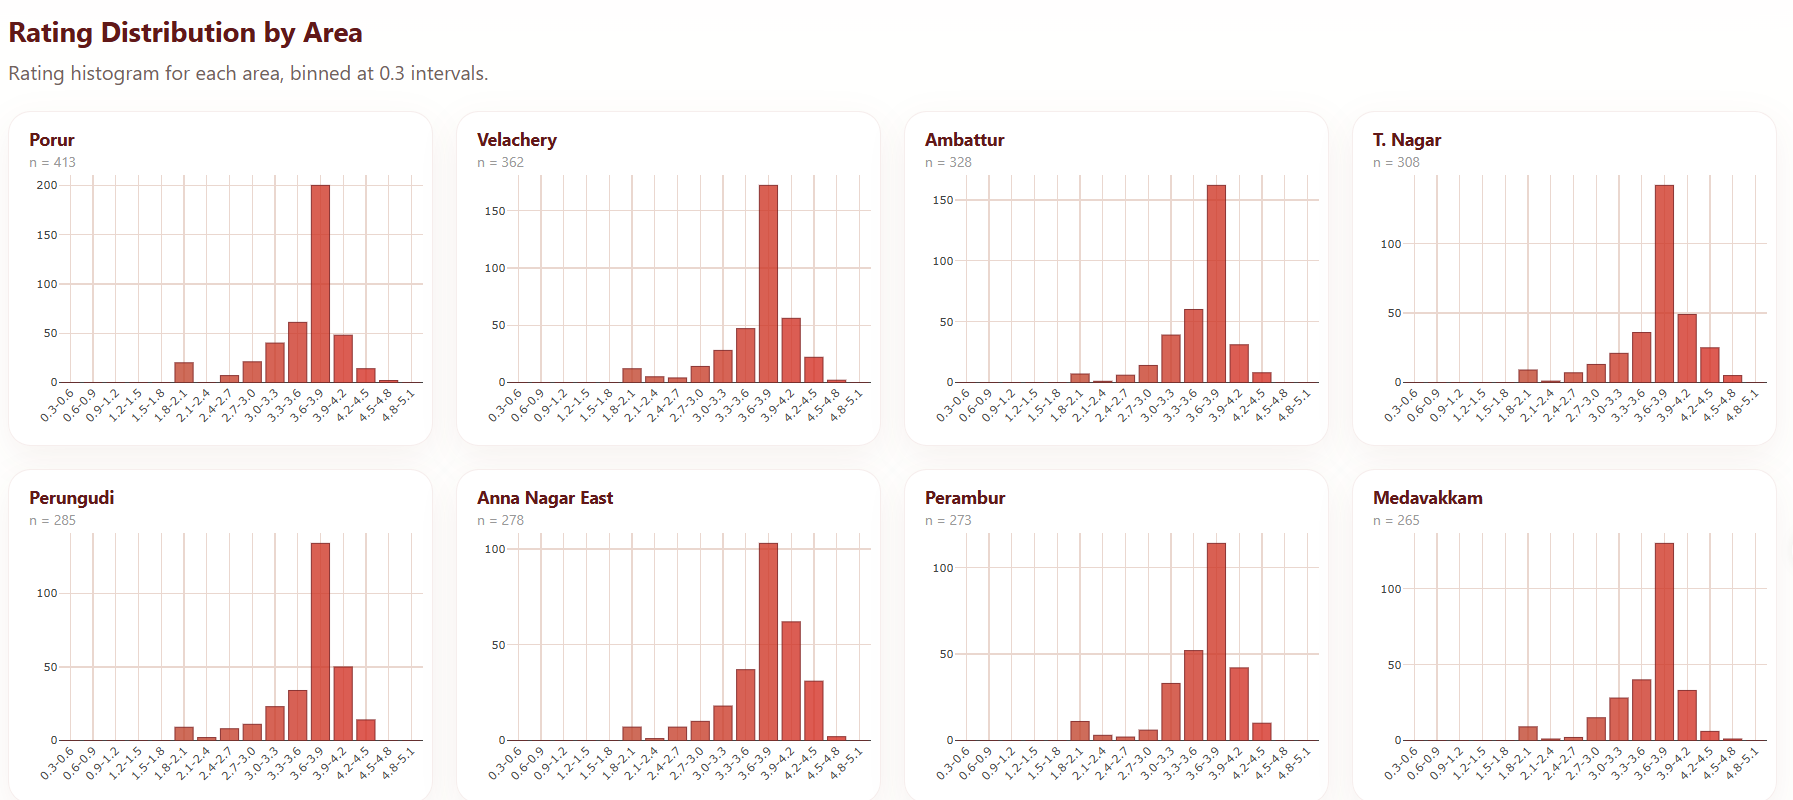
\includegraphics[width=0.95\textwidth]{figures/11_area_histogram.png}
\caption{区域评分直方图}
\label{fig:area_histogram}
\end{figure}

图~\ref{fig:area_histogram} 展示了主要区域的评分分布对比。通过分面展示不同区域的评分直方图，可以快速识别哪些区域的评分整体偏高，哪些区域存在较大的评分波动。

\begin{figure}[H]
\centering
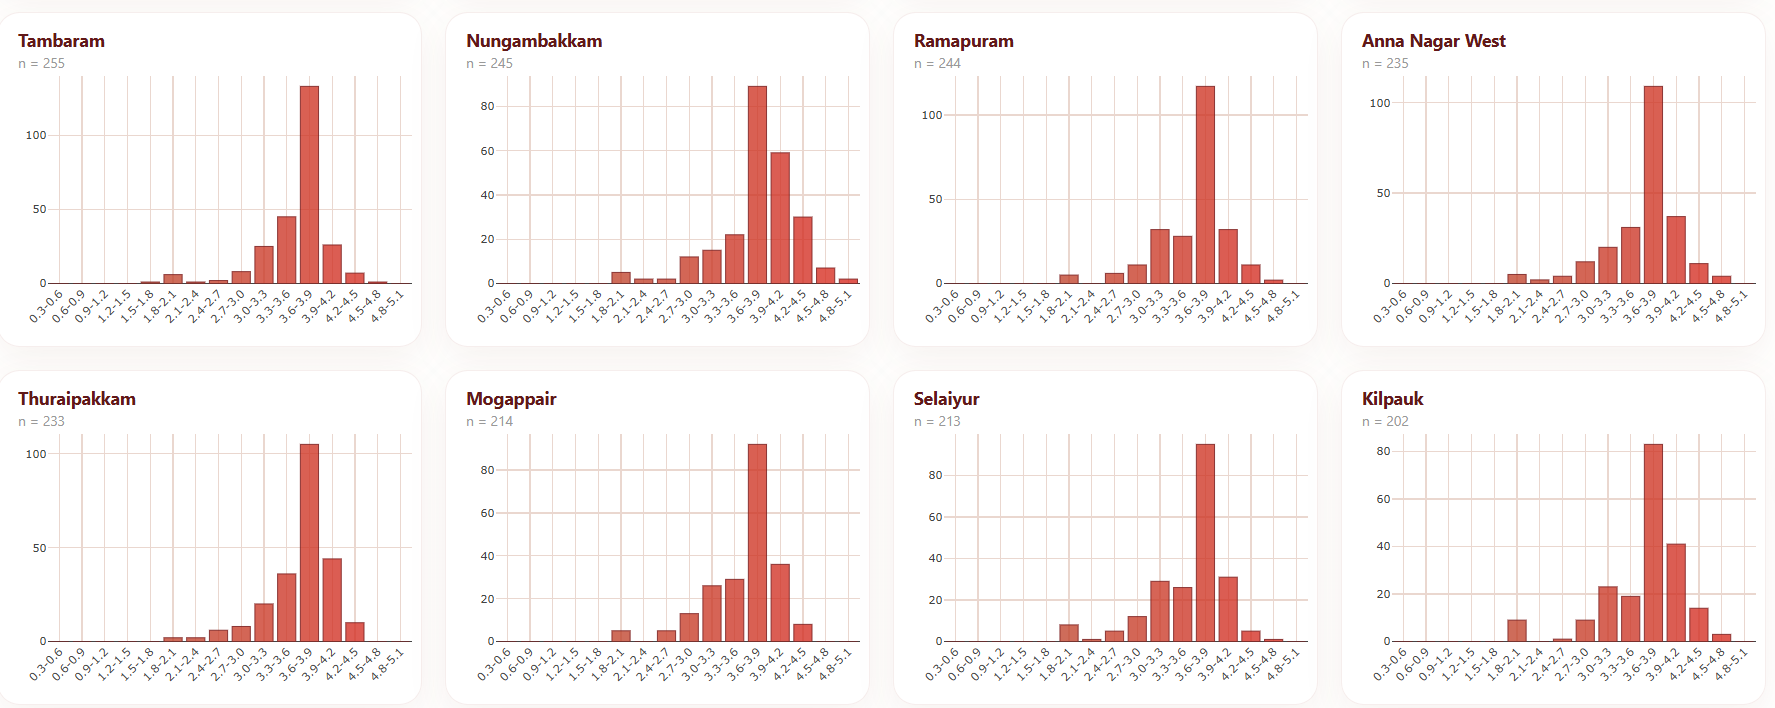
\includegraphics[width=0.95\textwidth]{figures/12_area_histogram_top.png}
\caption{Top 区域评分分布对比}
\label{fig:area_top_histogram}
\end{figure}

图~\ref{fig:area_top_histogram} 进一步聚焦于门店数量较多的 Top 区域，通过更细粒度的分布对比，揭示不同区域在评分集中度和离散程度上的差异。

\subsection{菜系、菜品与服务特征分析}

从长格式拆分结果来看，Chinese、South Indian、North Indian 等菜系出现频次较高，本地菜如 Biryani、Dosa、Idli 等兼具较高覆盖率和较强地方文化特征。服务特色方面，Home Delivery 和 Indoor Seating 是最常见的两个特征，表明线上配送与线下堂食是平台餐厅服务供给的双核心。

\begin{figure}[H]
\centering
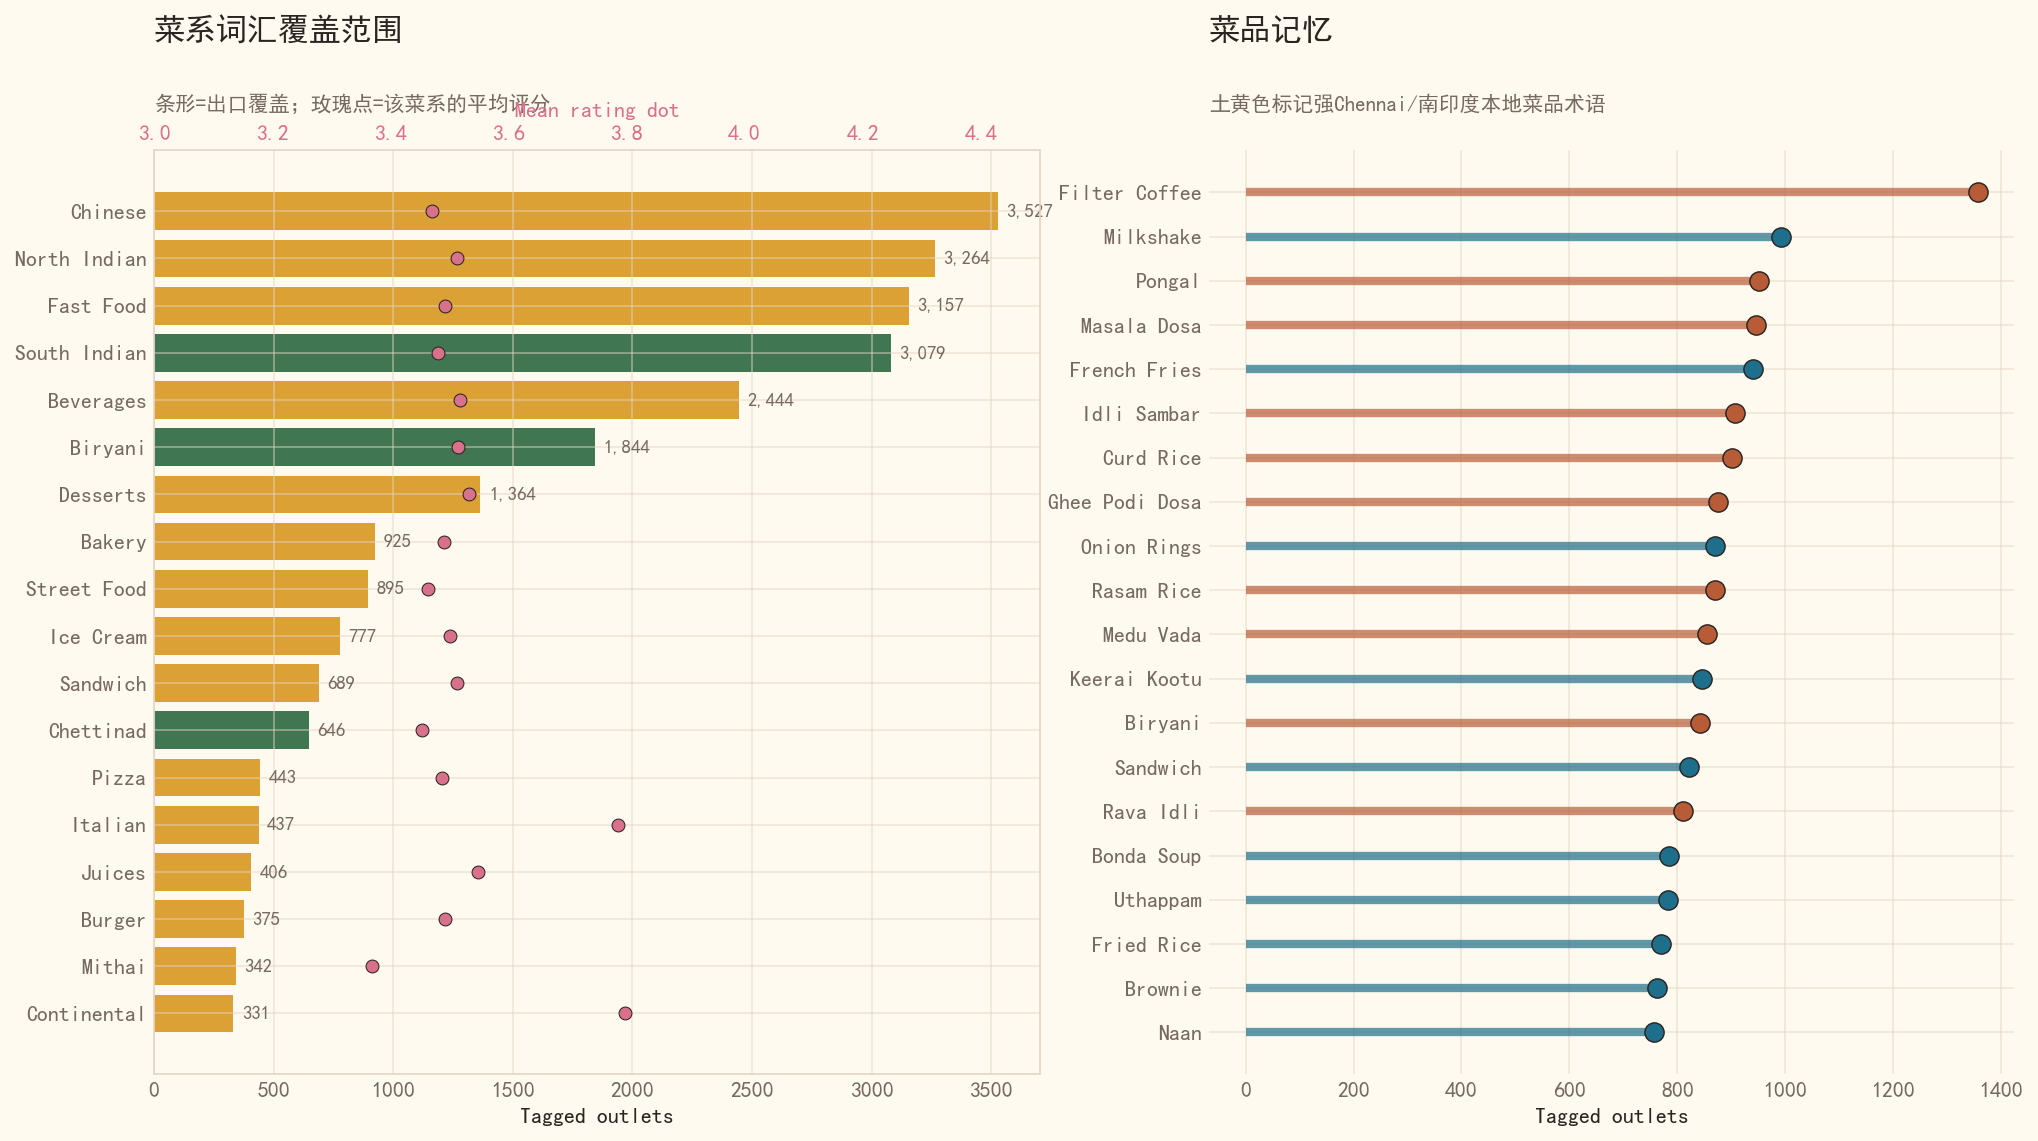
\includegraphics[width=0.95\textwidth]{figures/04_cuisine_and_dishes.png}
\caption{高频菜系与招牌菜分析}
\label{fig:cuisine_dish}
\end{figure}

图~\ref{fig:cuisine_dish} 中，条形图与散点图组合展示了菜系覆盖率与平均评分，棒棒糖式结构则突出本地菜品的出现频率。

\begin{figure}[H]
\centering
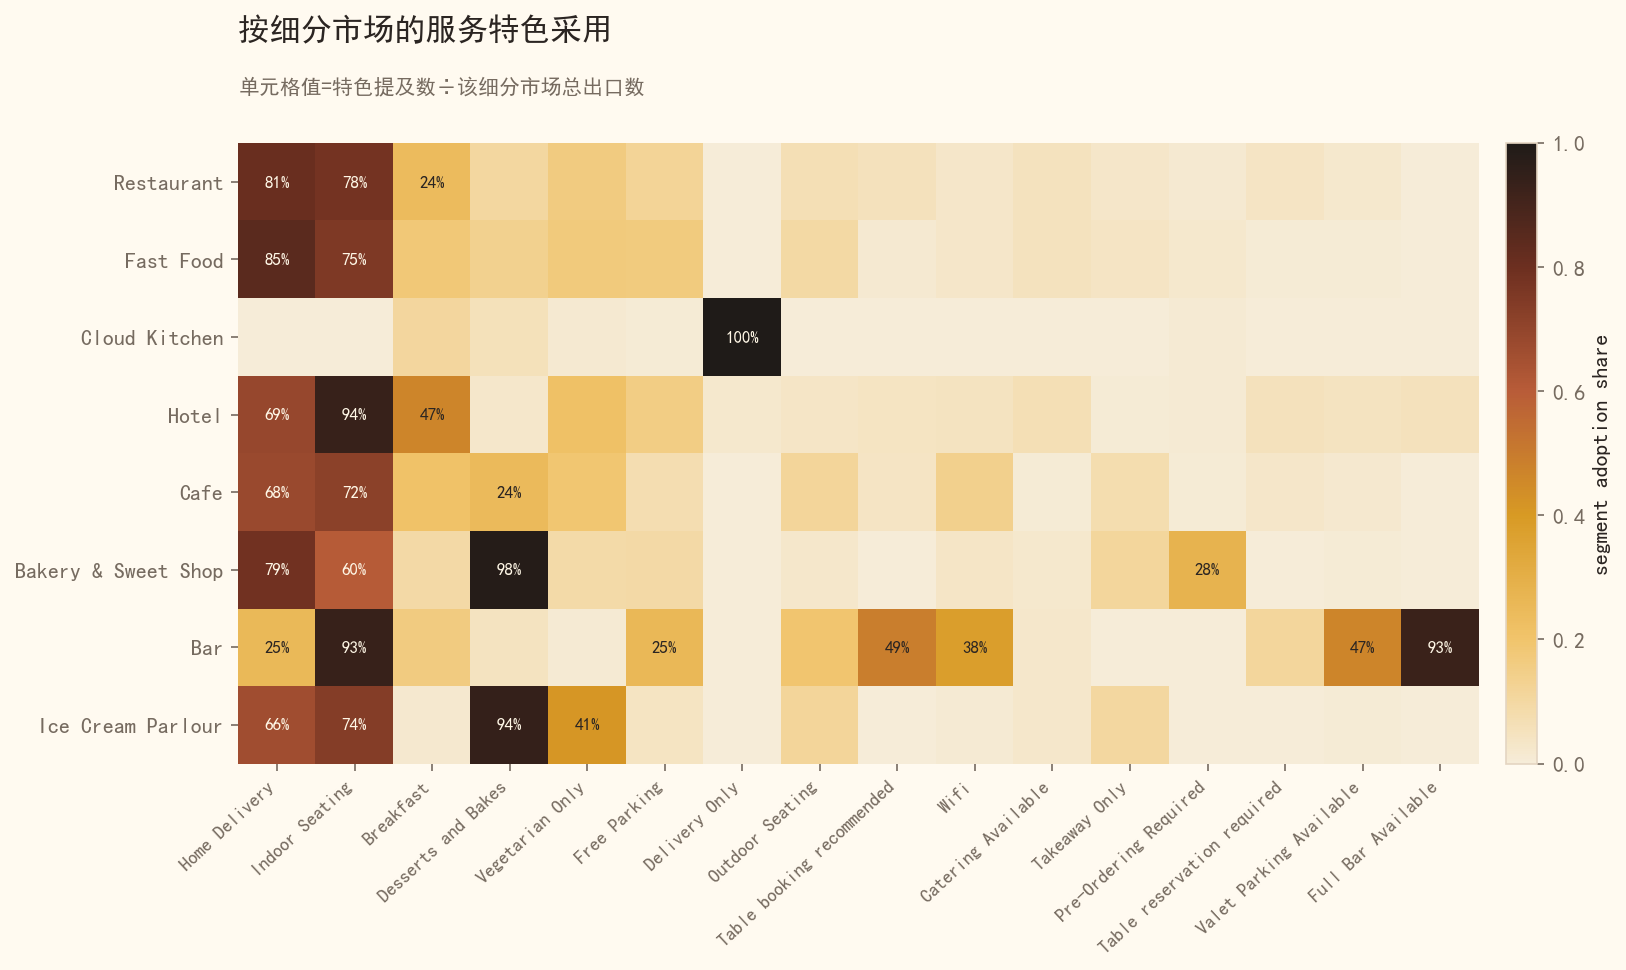
\includegraphics[width=0.95\textwidth]{figures/05_feature_heatmap.png}
\caption{不同市场细分的服务特色采用率热力图}
\label{fig:heatmap}
\end{figure}

图~\ref{fig:heatmap} 通过矩阵形式展示各市场细分对服务特色的采用比例。单元格值 = 特色提及数 / 该细分市场总门店数。可以看到，高频服务特征在不同业态中的分布并不均匀，这说明平台上的经营模式与消费者体验存在较强耦合关系。

\subsection{Segment 对评分影响的深入分析}

为了更深入地理解市场细分对评分的影响，本节通过多种可视化手段进行多角度分析。

\begin{figure}[H]
\centering
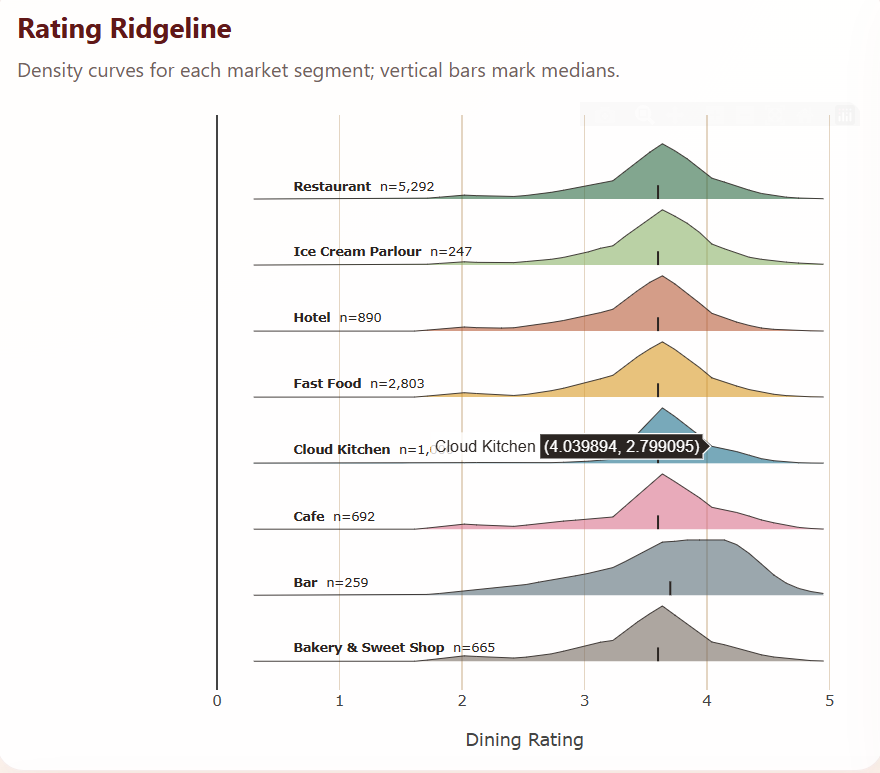
\includegraphics[width=0.95\textwidth]{figures/21_rating_ridgelines_segment.png}
\caption{市场细分评分脊线分布（EDA 交互界面）}
\label{fig:ridgelines_segment}
\end{figure}

图~\ref{fig:ridgelines_segment} 使用脊线图对不同市场细分的评分分布进行横向比较。每条密度曲线代表一个细分市场的评分分布，竖线标记中位数位置。通过脊线图可以直观地看到：Cloud Kitchen 的评分分布整体偏右（高分），而部分传统业态的分布则更为分散。

\begin{figure}[H]
\centering
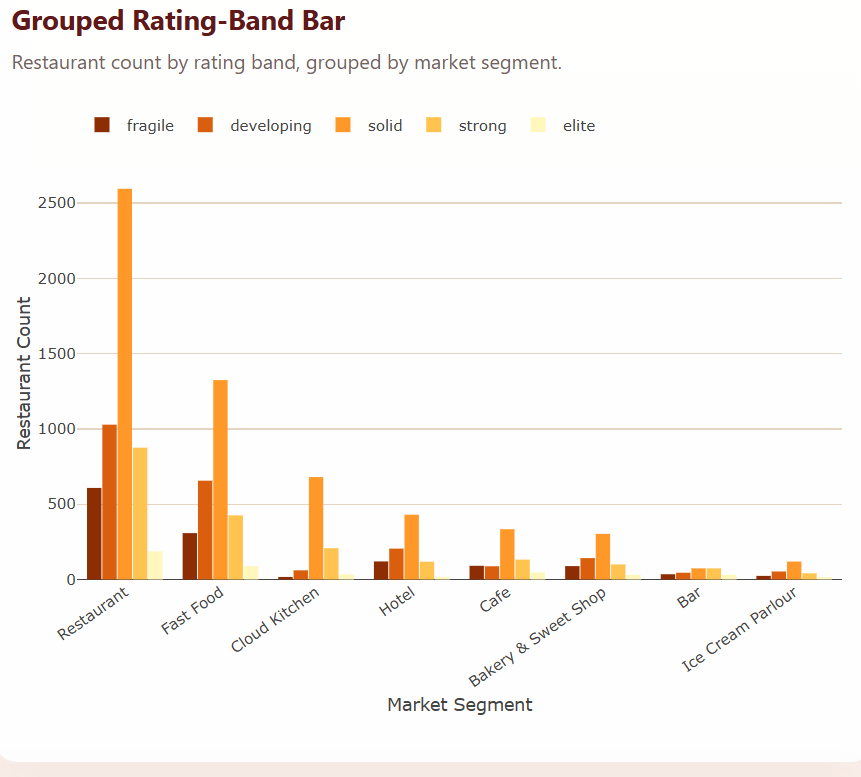
\includegraphics[width=0.95\textwidth]{figures/20_grouped_bar_rating.png}
\caption{按评分分级的市场分组柱形图}
\label{fig:grouped_bar}
\end{figure}

图~\ref{fig:grouped_bar} 以评分分级（rating\_band）作为分组变量，对比不同市场细分在各评分等级下的门店数量。这种分组柱形图可以揭示不同业态在评分等级构成上的差异。

\begin{figure}[H]
\centering
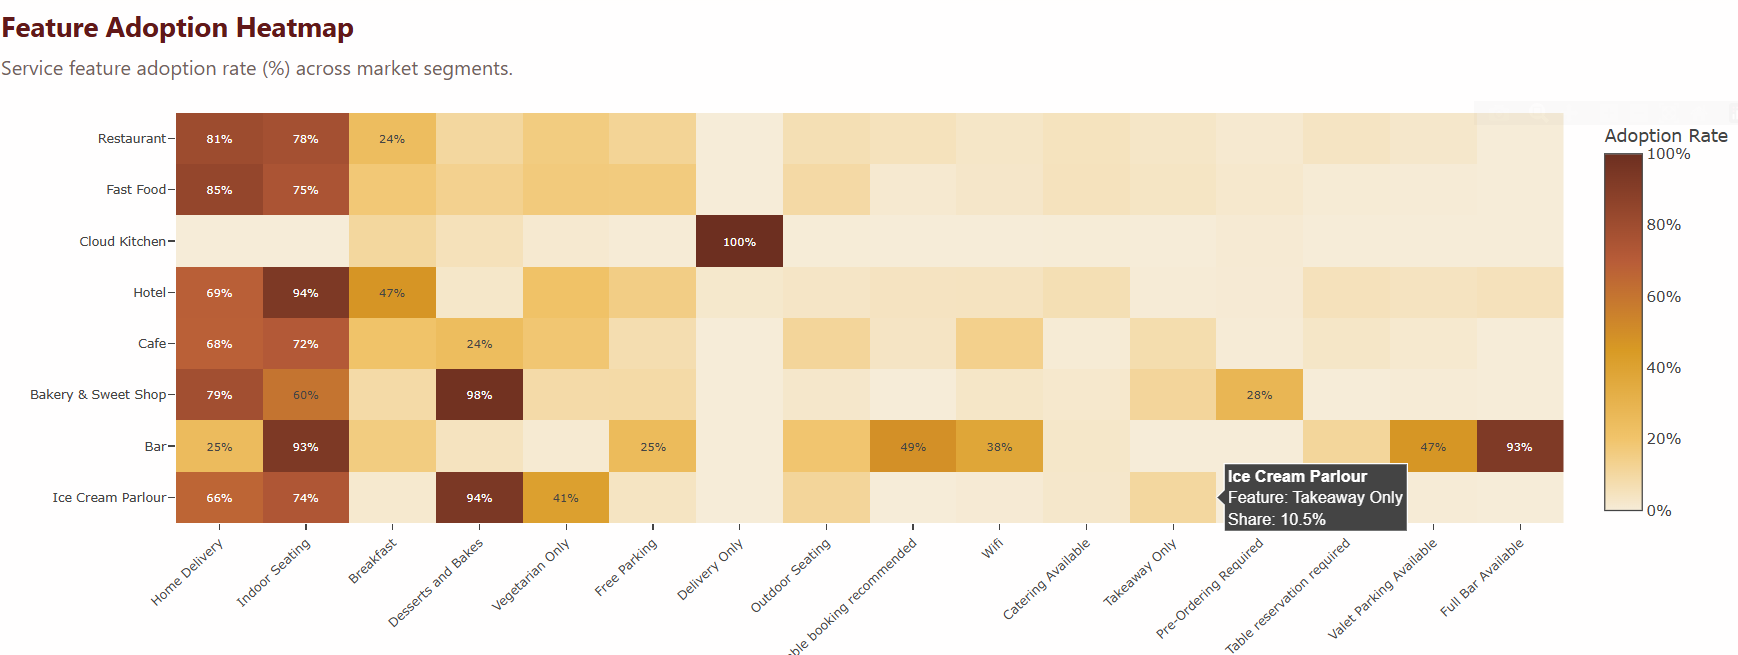
\includegraphics[width=0.95\textwidth]{figures/22_feature_heatmap_segment.png}
\caption{菜系结构与服务特色比例热力图}
\label{fig:cuisine_feature_heatmap}
\end{figure}

图~\ref{fig:cuisine_feature_heatmap} 展示了菜系结构与服务特色之间的关联。通过百分比矩阵形式，可以观察到不同菜系对各类服务特色的采用比例差异，从而洞察菜系文化与服务模式之间的耦合关系。

\begin{figure}[H]
\centering
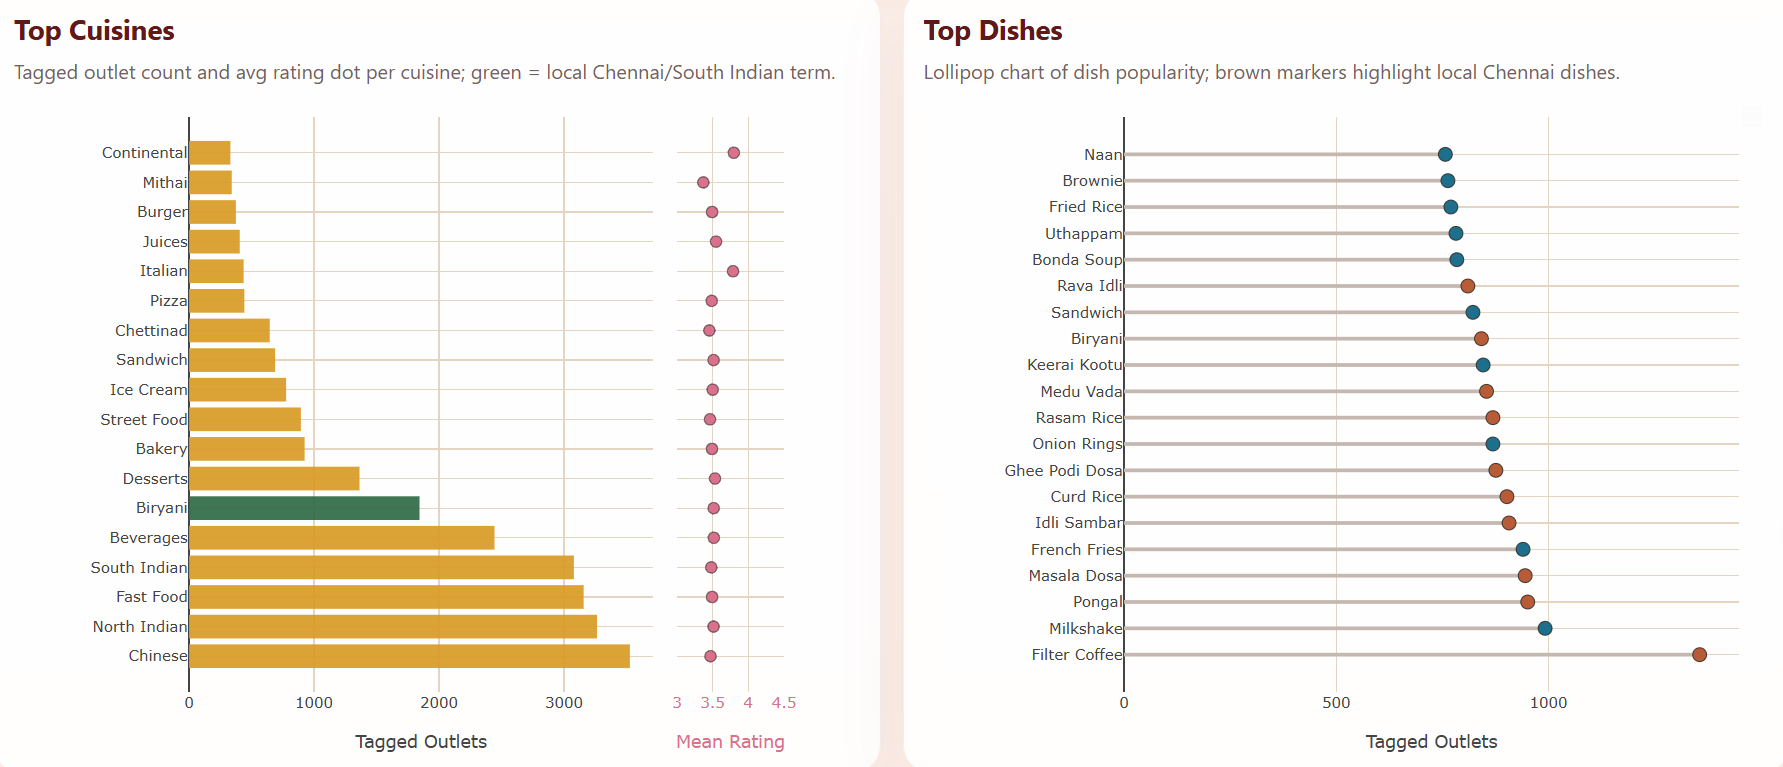
\includegraphics[width=0.95\textwidth]{figures/23_popular_dishes.png}
\caption{最受喜爱的菜品与地方特色菜品分析}
\label{fig:popular_dishes}
\end{figure}

图~\ref{fig:popular_dishes} 聚焦于菜品维度的分析，展示了最受欢迎的菜品和具有地方文化特色的菜品。Biryani、Dosa、Idli、Filter Coffee 等本地菜品在覆盖率和评分上均表现突出，体现了 Chennai 餐饮市场深厚的本地饮食文化底蕴。

\subsection{区域空间分布与机会识别}

从区域尺度看，Chennai 餐饮市场呈现明显的空间异质性。部分区域门店极度密集，但平均评分并不占优；另一些区域供给规模有限，却拥有更高的平均评分。

\begin{figure}[H]
\centering
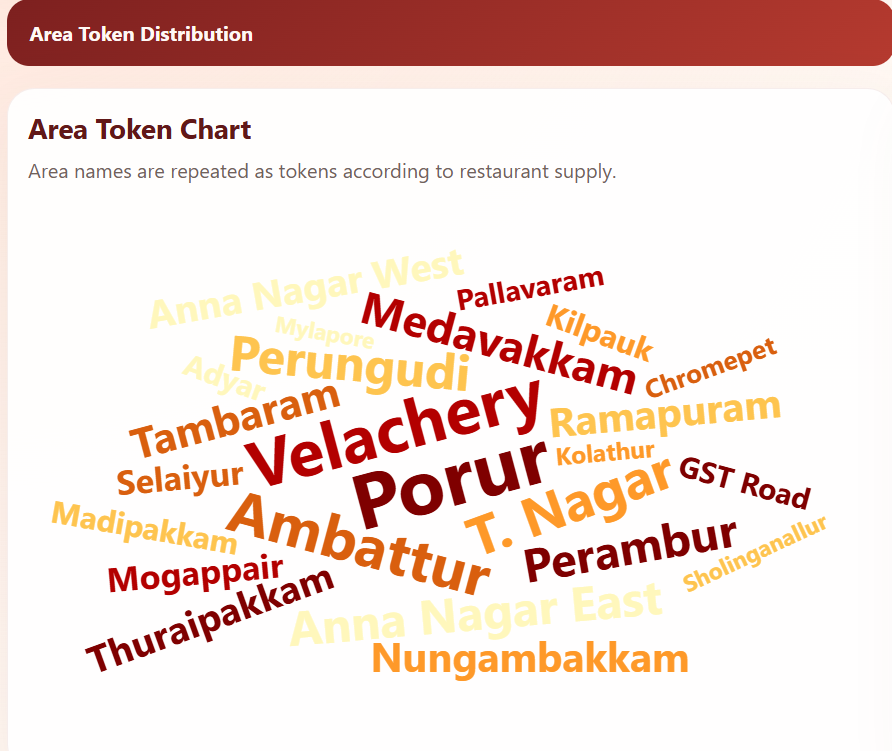
\includegraphics[width=0.95\textwidth]{figures/24_area_wordcloud.png}
\caption{区域名称词云图}
\label{fig:wordcloud}
\end{figure}

图~\ref{fig:wordcloud} 使用词云图展示了区域名称的频率分布。词云中字体越大的区域名代表该区域的餐厅数量越多。从词云中可以直观地识别出 Chennai 的核心餐饮商圈。

\begin{figure}[H]
\centering
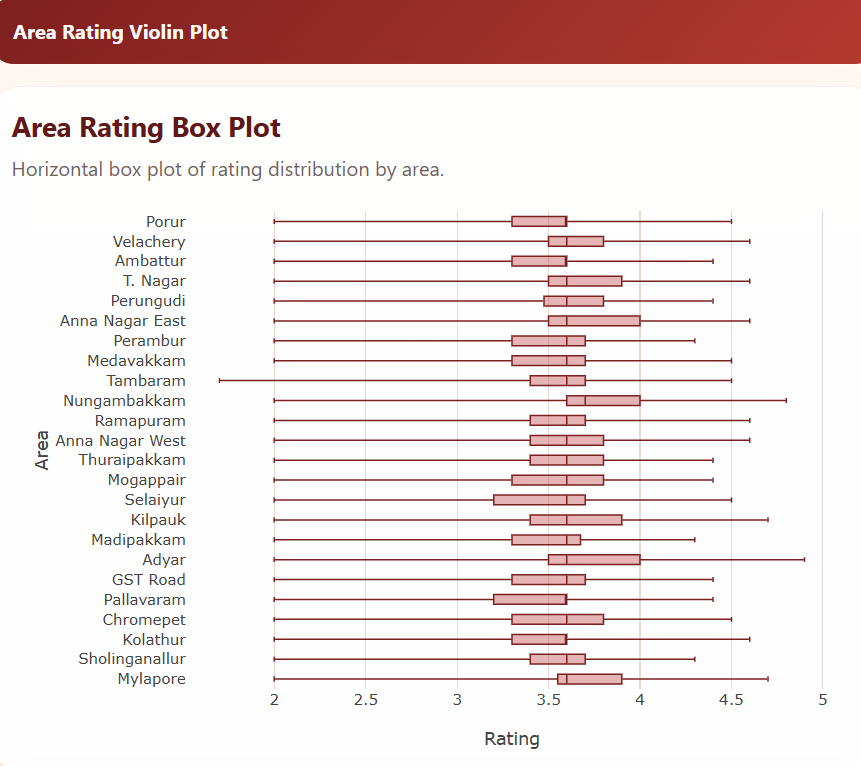
\includegraphics[width=0.95\textwidth]{figures/25_area_boxplot.png}
\caption{不同区域评分箱线图}
\label{fig:boxplot}
\end{figure}

图~\ref{fig:boxplot} 使用箱线图比较不同区域的评分分布。箱线图的优势在于能够同时展示中位数、四分位间距和异常值，适合识别评分分布的稳健特征和异常情况。

\begin{figure}[H]
\centering
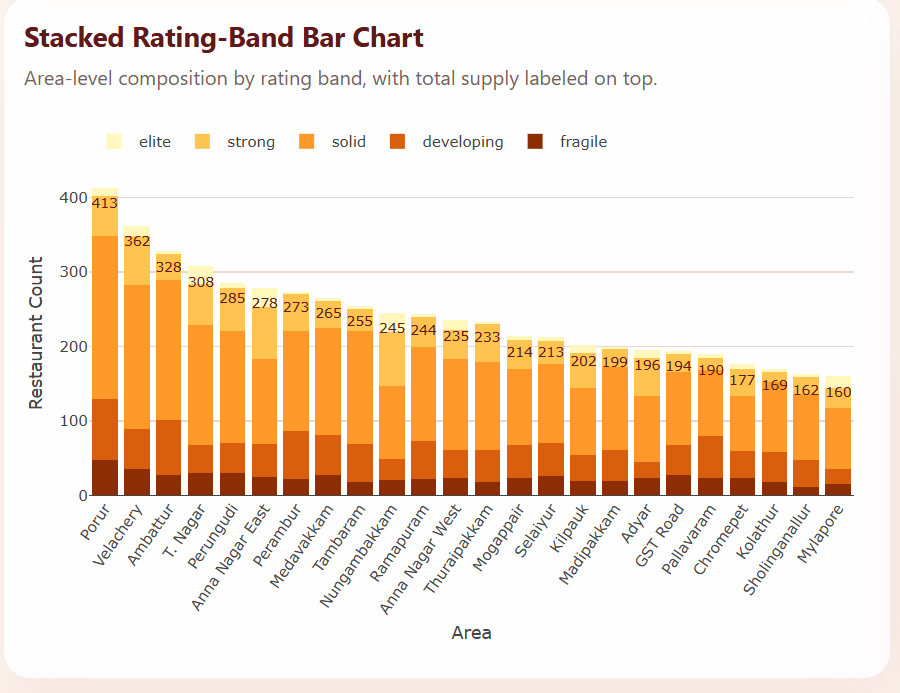
\includegraphics[width=0.95\textwidth]{figures/26_area_stacked_bar.png}
\caption{区域评分分级堆叠柱形图}
\label{fig:stacked_bar}
\end{figure}

图~\ref{fig:stacked_bar} 使用堆叠柱形图比较不同区域在五档 rating\_band 下的结构差异。通过堆叠比例可以快速识别哪些区域的"elite"级餐厅占比更高，哪些区域的"fragile"级餐厅需要改进。

\begin{figure}[H]
\centering
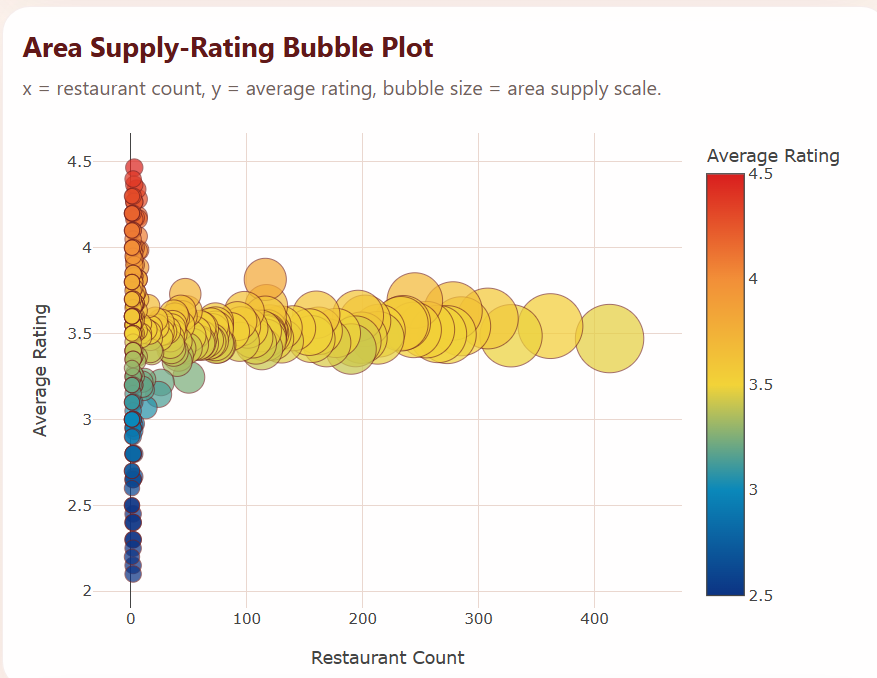
\includegraphics[width=0.95\textwidth]{figures/27_area_bubble.png}
\caption{区域气泡图：供给量 vs 评分 vs 区域规模}
\label{fig:bubble}
\end{figure}

图~\ref{fig:bubble} 使用气泡图同时展示三个维度：X 轴为餐厅数量（供给），Y 轴为平均评分，气泡大小代表区域规模。这种多维组合图可以同时观察供给密度、评分水平和区域规模三者之间的关系。

\begin{figure}[H]
\centering
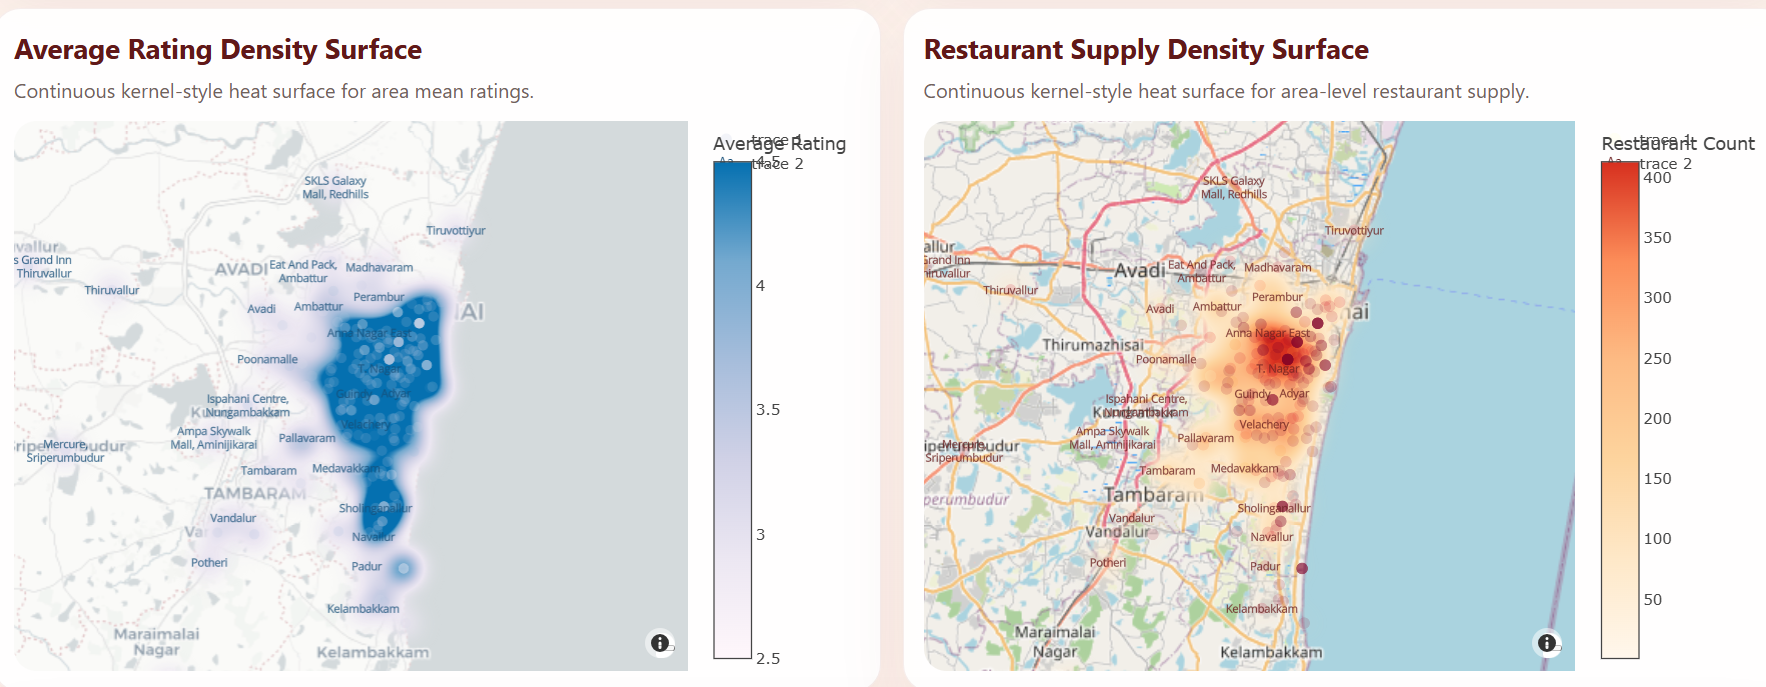
\includegraphics[width=0.95\textwidth]{figures/28_kde_heatmap.png}
\caption{核密度估计热力图（餐厅数 vs 平均评分）}
\label{fig:kde}
\end{figure}

图~\ref{fig:kde} 使用核密度估计（KDE）生成空间热力分布。左图为平均评分的密度分布，右图为区域餐厅总数的密度分布。两图密度较高部分并不完全重合，反映出区域餐厅数并不是与平均分数具备完全正相关。同时可以观察到"沿海密集、内陆疏松"的分布格局。

\begin{figure}[H]
\centering
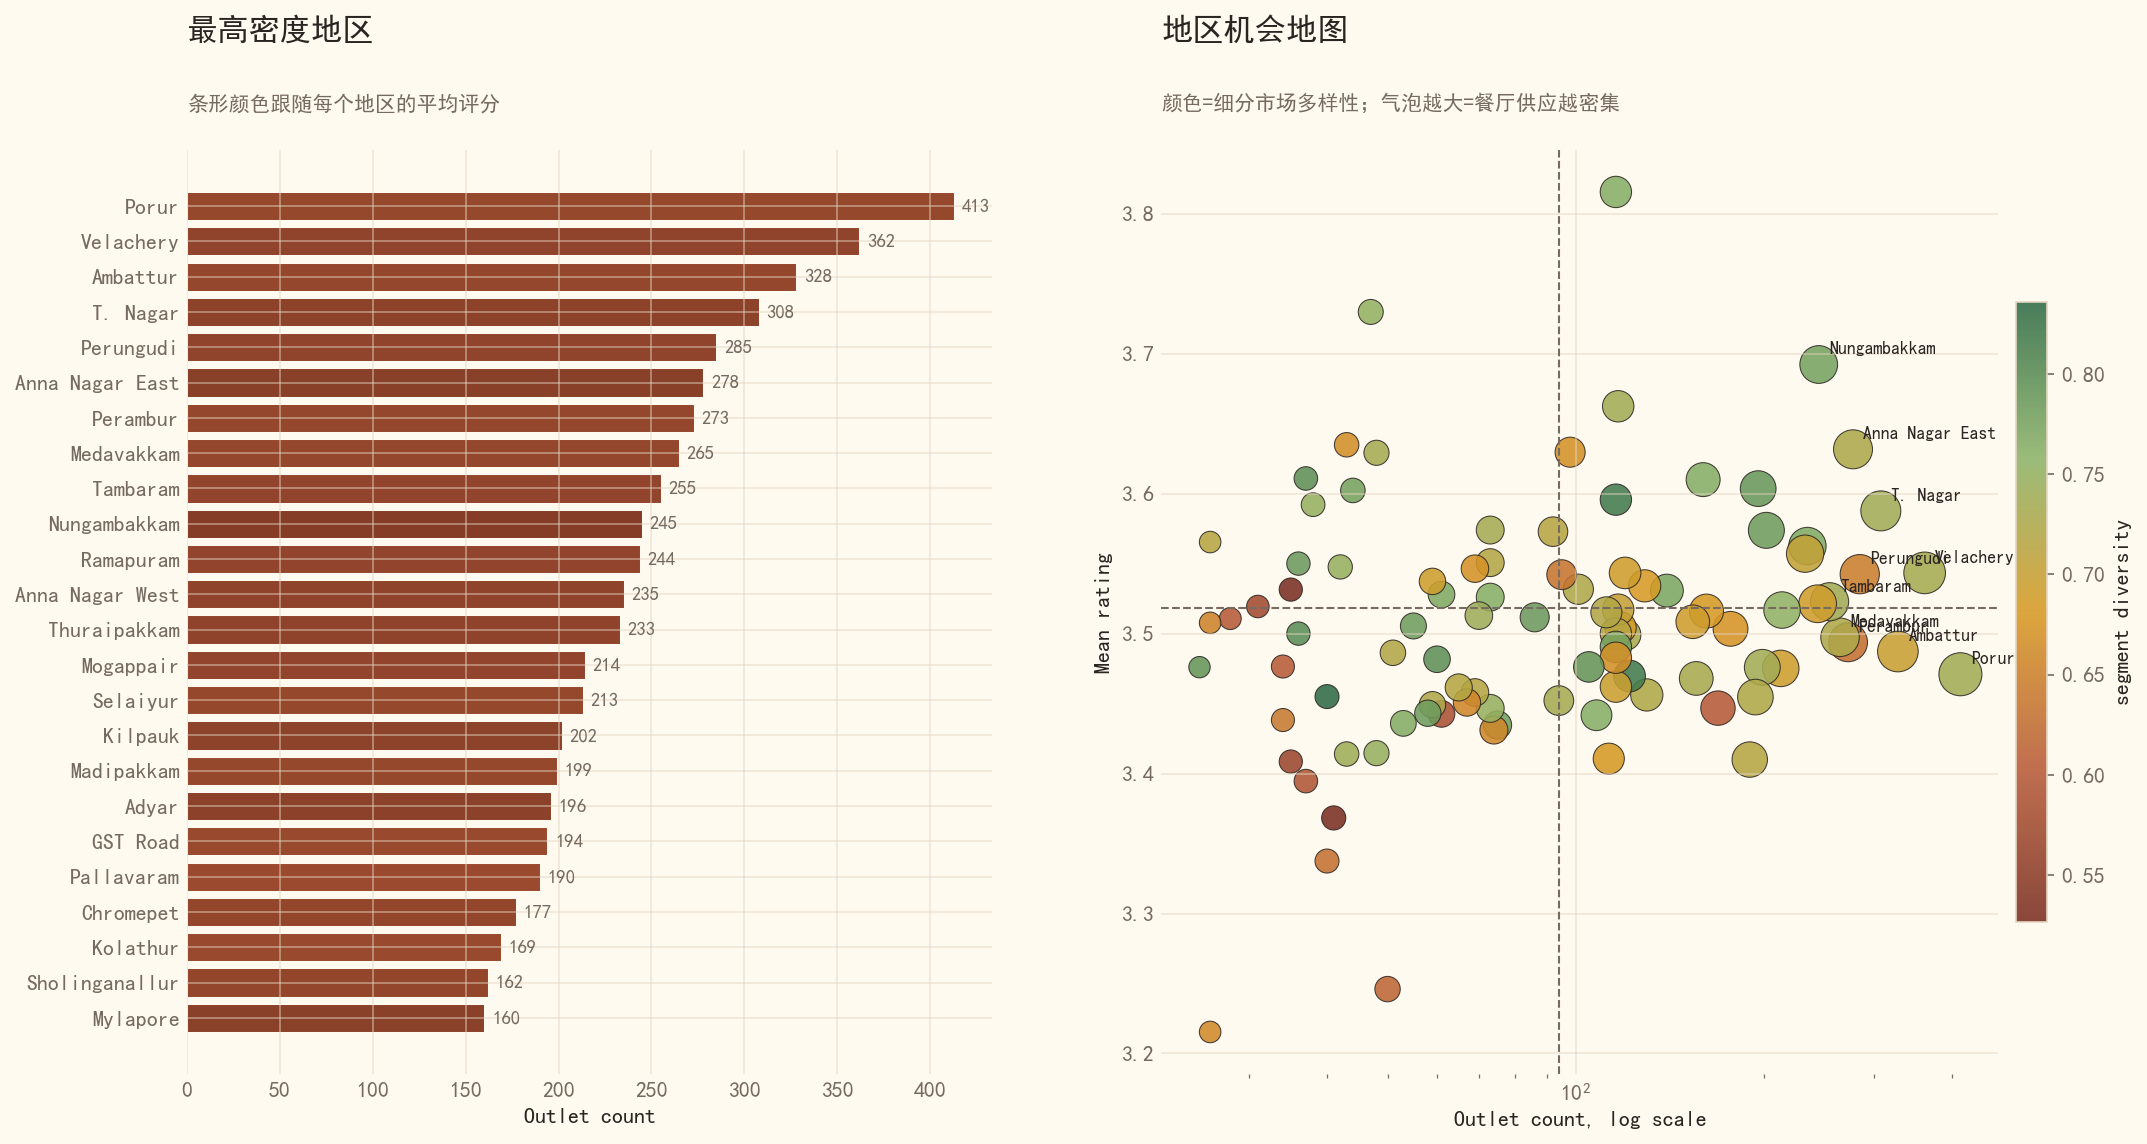
\includegraphics[width=0.95\textwidth]{figures/06_area_analysis.png}
\caption{区域供给量、评分与机会地图分析}
\label{fig:area}
\end{figure}

图~\ref{fig:area} 左图显示高密度区域的门店规模和评分差异，右图通过气泡散点图将餐厅数量、平均评分与细分多样性结合起来，为区域比较提供了更丰富的维度。

\begin{figure}[H]
\centering
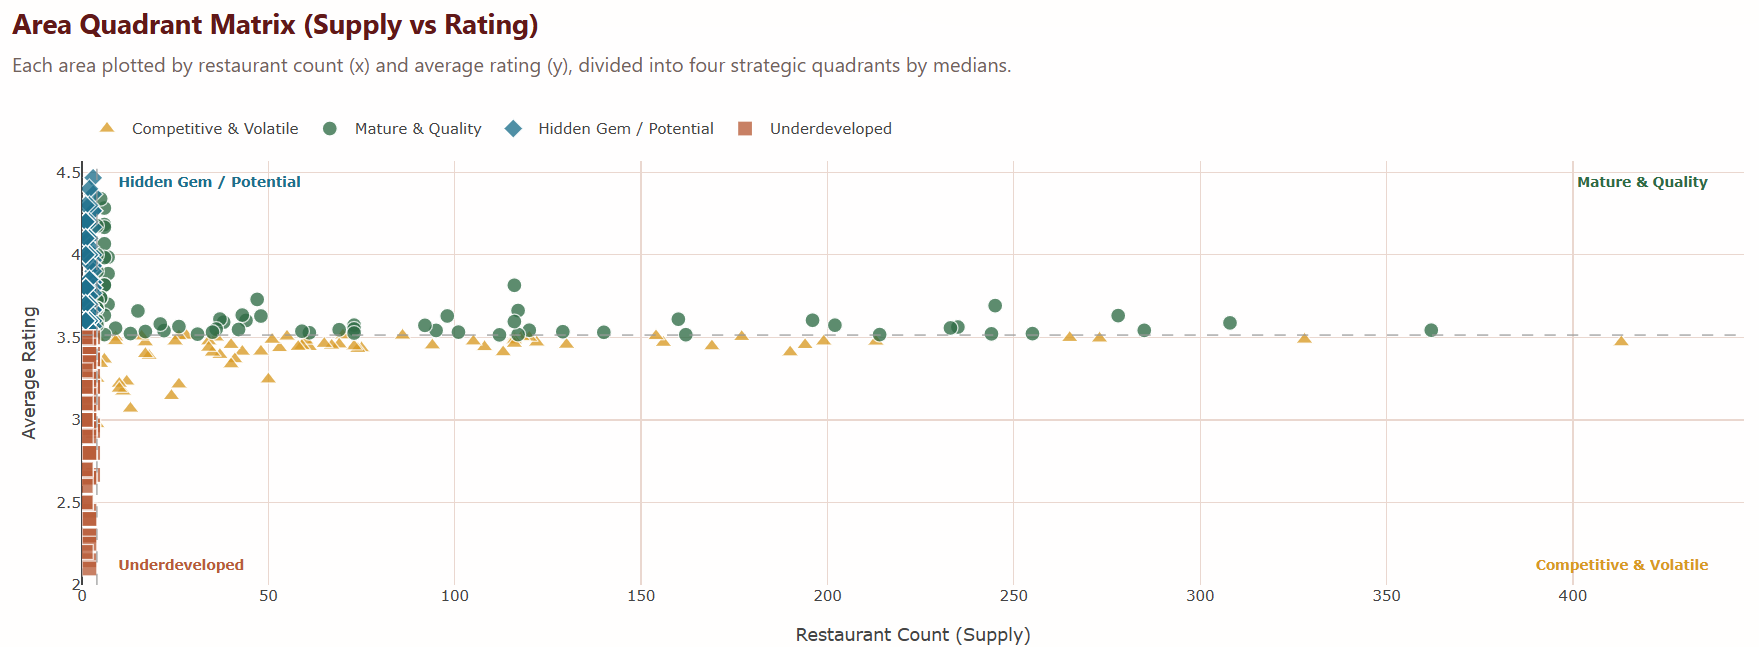
\includegraphics[width=0.95\textwidth]{figures/29_quadrant_matrix.png}
\caption{四象限矩阵图：供给密度 vs 平均评分}
\label{fig:quadrant}
\end{figure}

图~\ref{fig:quadrant} 是空间分析的核心图表之一。以区域餐厅数中位数（X 轴）和平均评分中位数（Y 轴）作为分界线，将所有区域划分为四类。从图中可以观察到：
\begin{itemize}[leftmargin=2em]
    \item 大量店铺聚集在 Y 轴附近，说明多数区域的供给量并不大；
    \item 连锁餐厅往往 rating 较高，私有餐厅具有"百花齐放"的态势；
    \item 右上象限（成熟优质区）中 T. Nagar 和 Anna Nagar 表现突出；
    \item 左上象限（潜力区）中存在一些评分较高但供给有限的区域，可能是蓝海机会。
\end{itemize}

\begin{figure}[H]
\centering
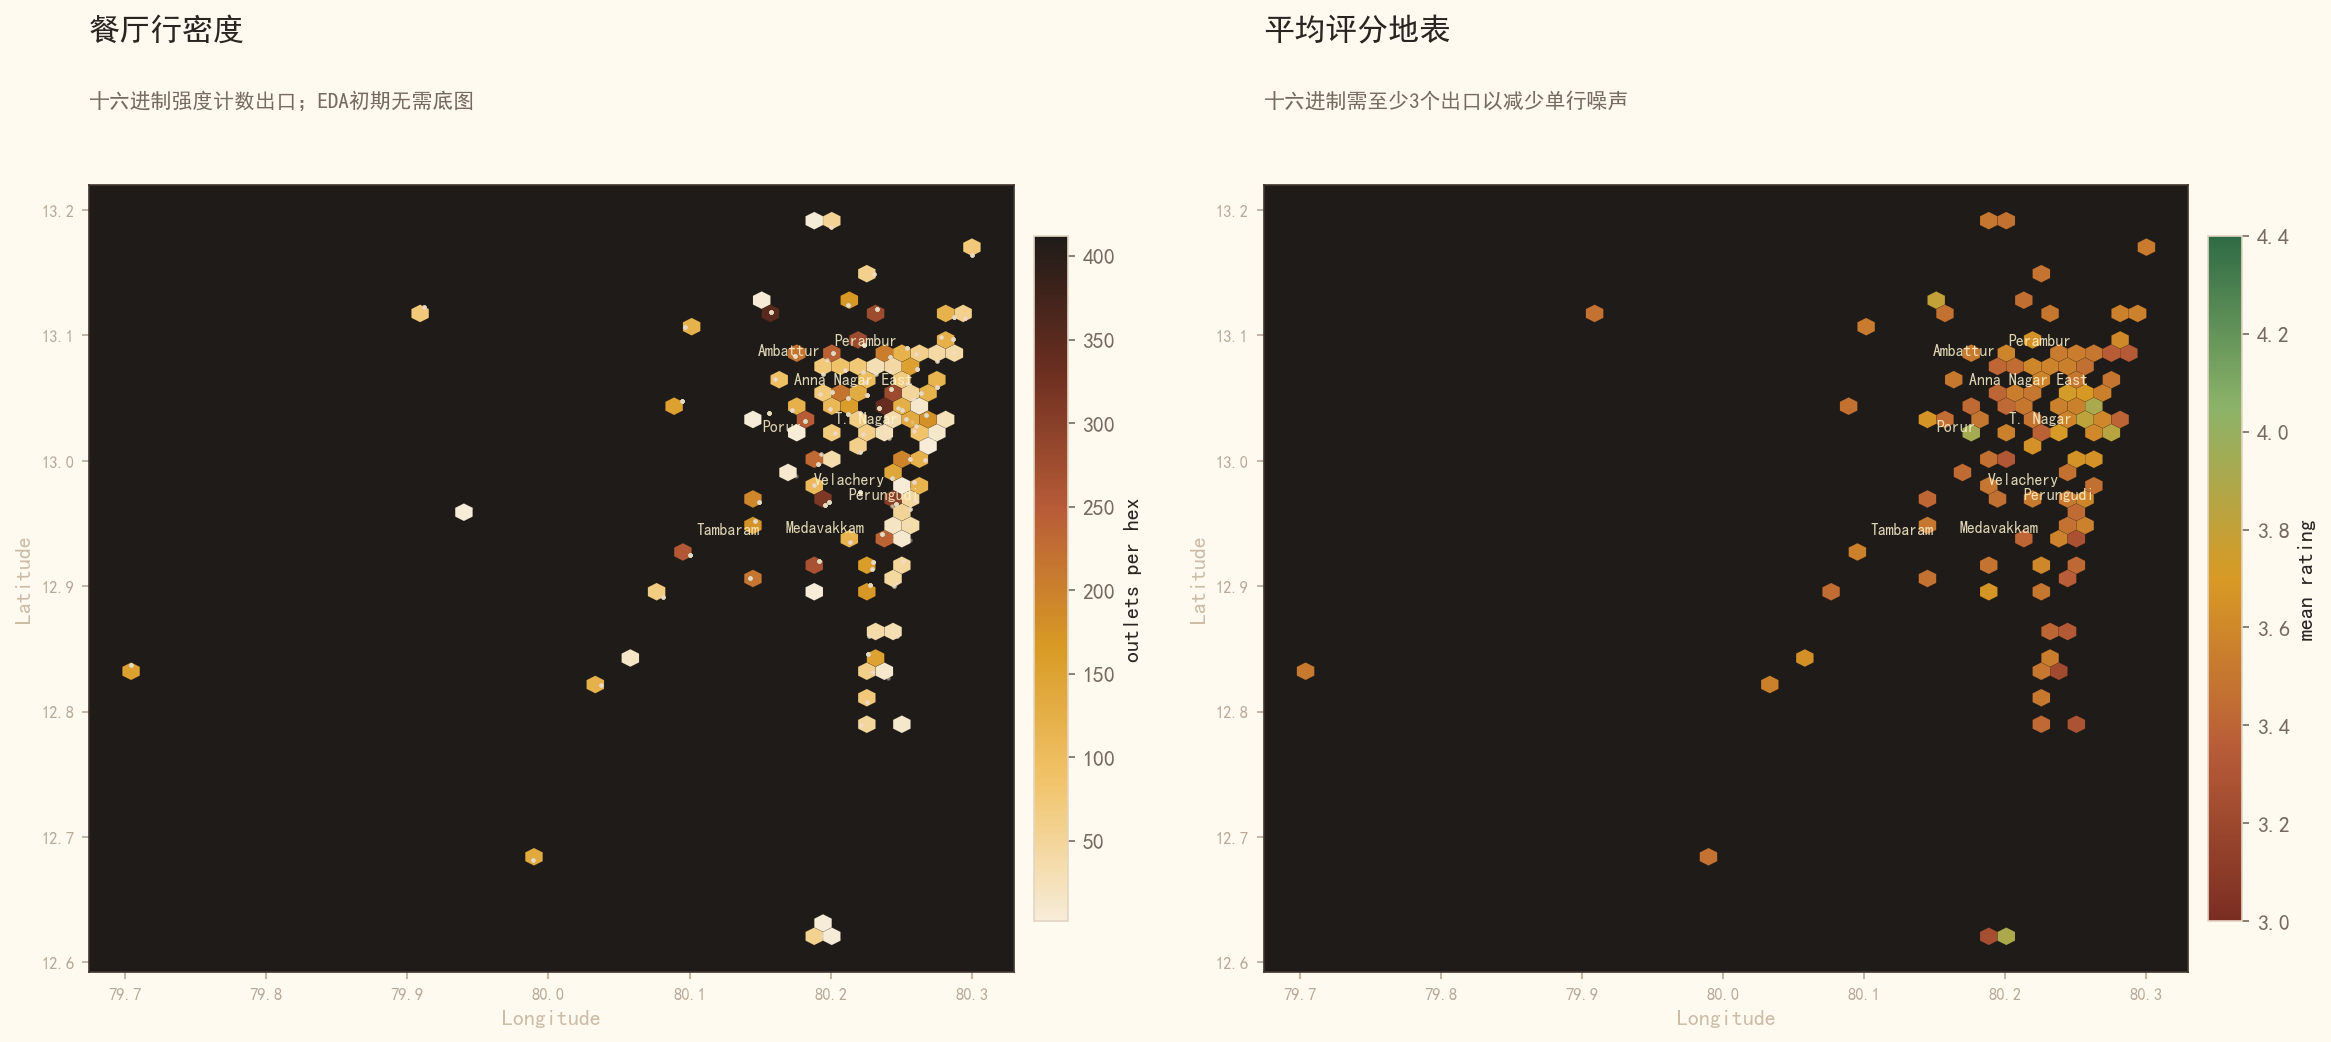
\includegraphics[width=0.95\textwidth]{figures/07_spatial_distribution.png}
\caption{餐厅空间密度与平均评分地表}
\label{fig:spatial}
\end{figure}

图~\ref{fig:spatial} 的空间热力图表明，餐厅供给的高密度区域与评分高值区域并不完全重合，这意味着"热闹区域"未必就是"高质量区域"。这一结果对商业选址和用户推荐都具有较强的应用价值。

\begin{table}[H]
\renewcommand{\arraystretch}{1.3}
\caption{四象限区域分类结果}
\label{tab:quadrant}
\centering
\begin{tabularx}{\textwidth}{lX}
\toprule
\textbf{象限} & \textbf{特征描述} \\
\midrule
Mature \& Quality & 高供给、高评分（如 T. Nagar、Anna Nagar）\\
Hidden Gem / Potential & 低供给、高评分（小而美/潜力区）\\
Competitive \& Volatile & 高供给、低评分（竞争激烈但质量不稳）\\
Underdeveloped & 低供给、低评分（待发展区）\\
\bottomrule
\end{tabularx}
\end{table}

\subsection{品牌足迹与评分预测分析}

项目不仅考察了静态统计和图形关系，还进一步用机器学习模型分析评分驱动因素。

\begin{figure}[H]
\centering
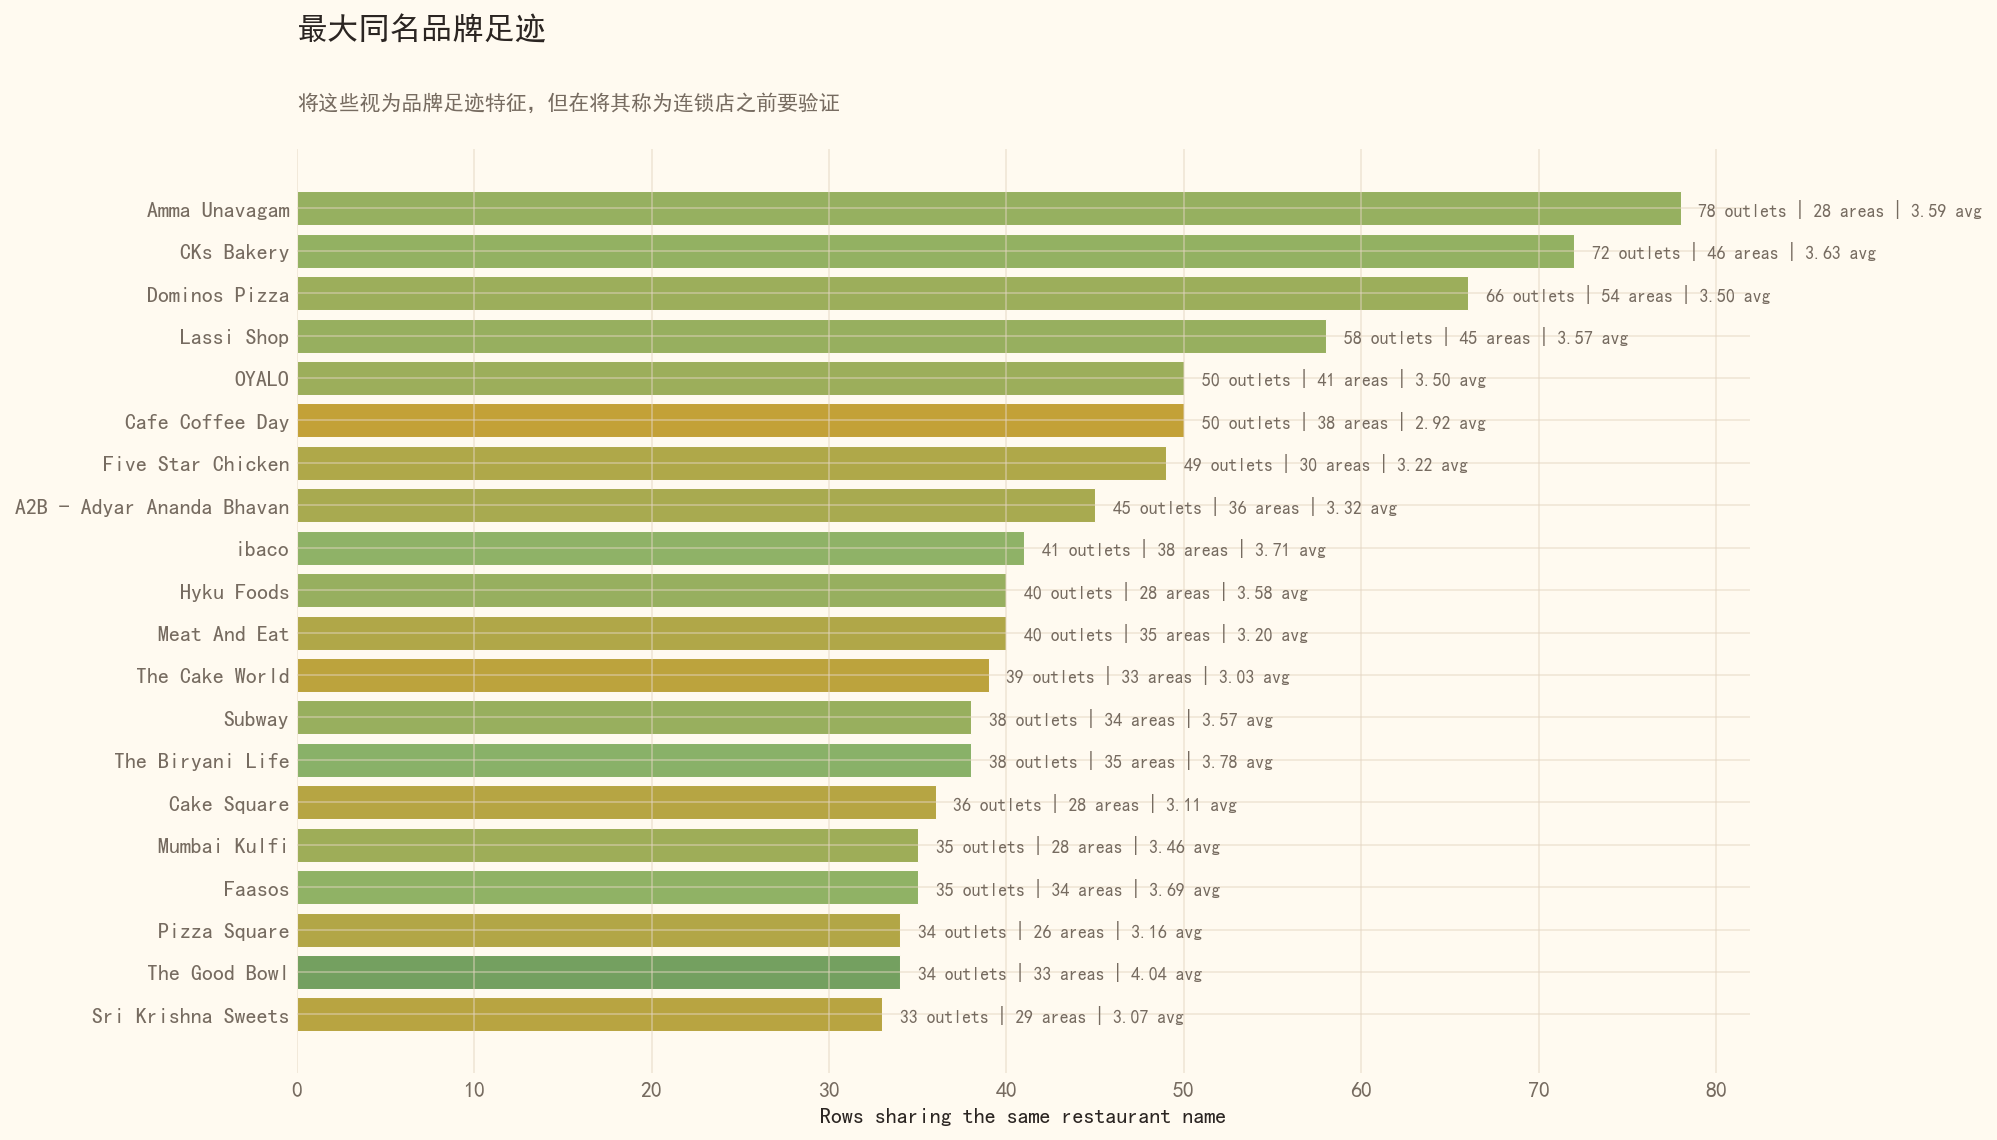
\includegraphics[width=0.95\textwidth]{figures/08_chain_footprints.png}
\caption{同名品牌足迹分析}
\label{fig:chain}
\end{figure}

图~\ref{fig:chain} 表明，多门店同名品牌在区域覆盖和平均评分上具有较强差异，这也为"品牌足迹是否影响评分"提供了分析切入点。

\subsubsection{模型对比与选择}

预测模块使用多种回归模型进行对比，评价指标包括 MAE（主要指标）、RMSE 和 $R^2$。模型对比结果如图~\ref{fig:model_leaderboard}所示。

\begin{figure}[H]
\centering
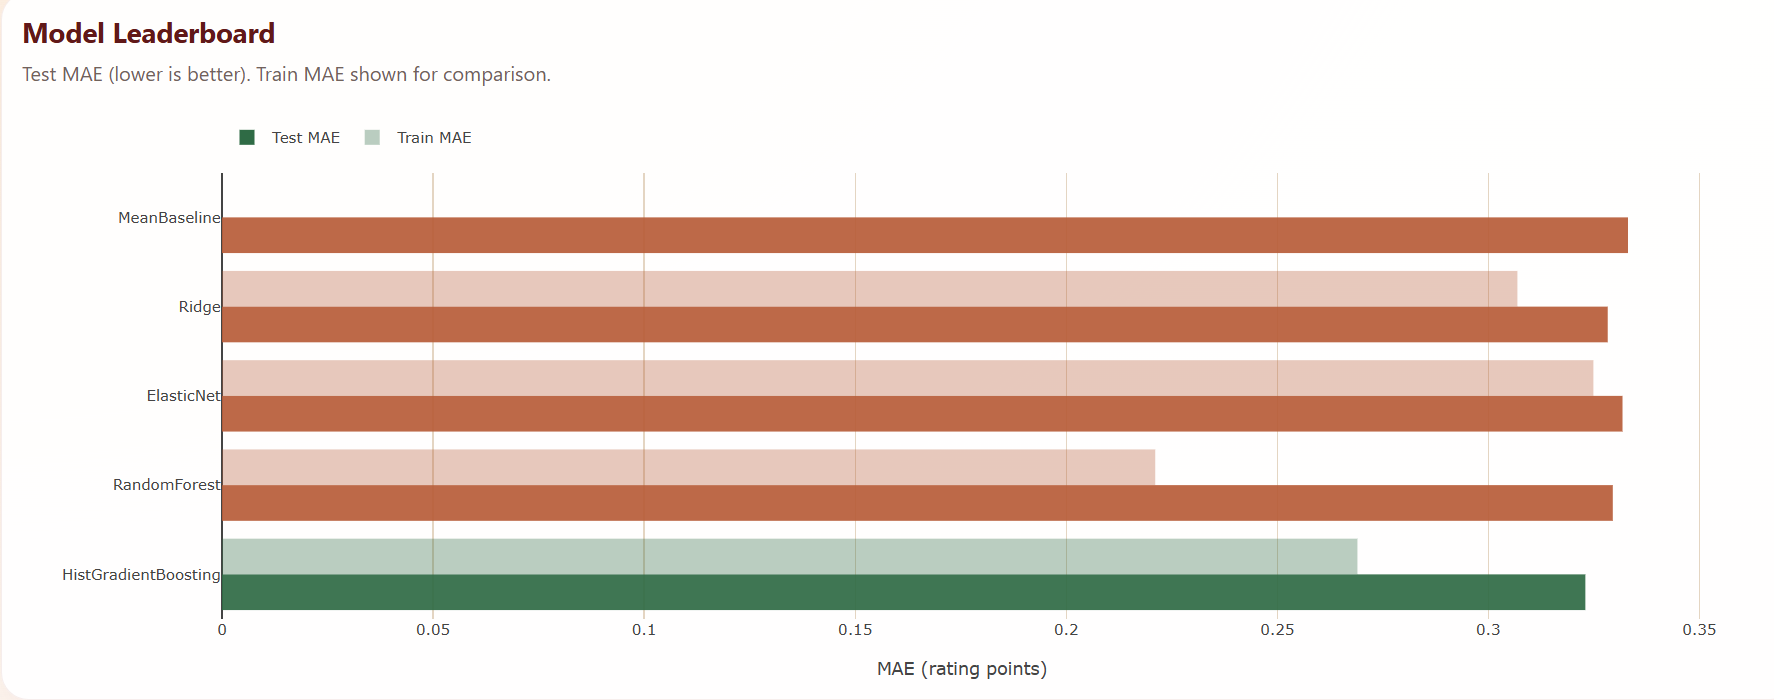
\includegraphics[width=0.95\textwidth]{figures/13_model_leaderboard.png}
\caption{模型排行榜：MAE / RMSE / $R^2$ 对比}
\label{fig:model_leaderboard}
\end{figure}

从模型排行榜中可以看到，从 DummyRegressor 基线到 HistGradientBoosting，模型性能逐步提升。最佳模型以 MAE 为准进行选择。

\subsubsection{残差分析与误差分解}

残差分析是理解模型预测质量的重要手段。

\begin{figure}[H]
\centering
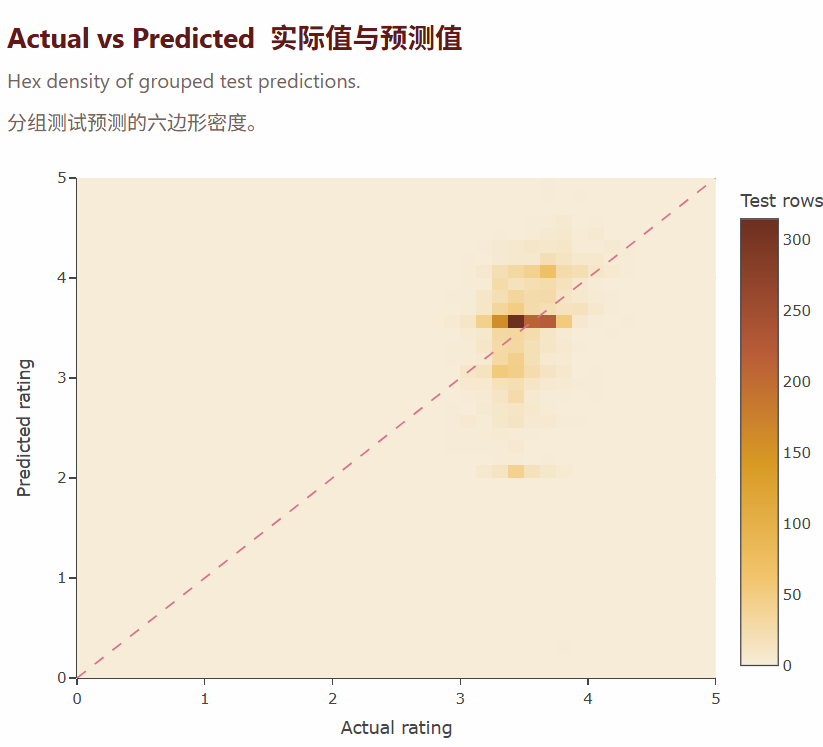
\includegraphics[width=0.95\textwidth]{figures/14_hexbin_density.png}
\caption{六边形密度图：实际评分 vs 预测评分}
\label{fig:hexbin}
\end{figure}

图~\ref{fig:hexbin} 使用六边形密度图展示实际评分与预测评分的关系。对角线虚线为完美预测参考线。六边形颜色深度表示该区域的数据点密度。从图中可以看到，预测值与实际值在 3.0--4.0 区间内拟合较好，但在极端值区域（低于 2.5 或高于 4.5）预测偏差较大。

\begin{figure}[H]
\centering
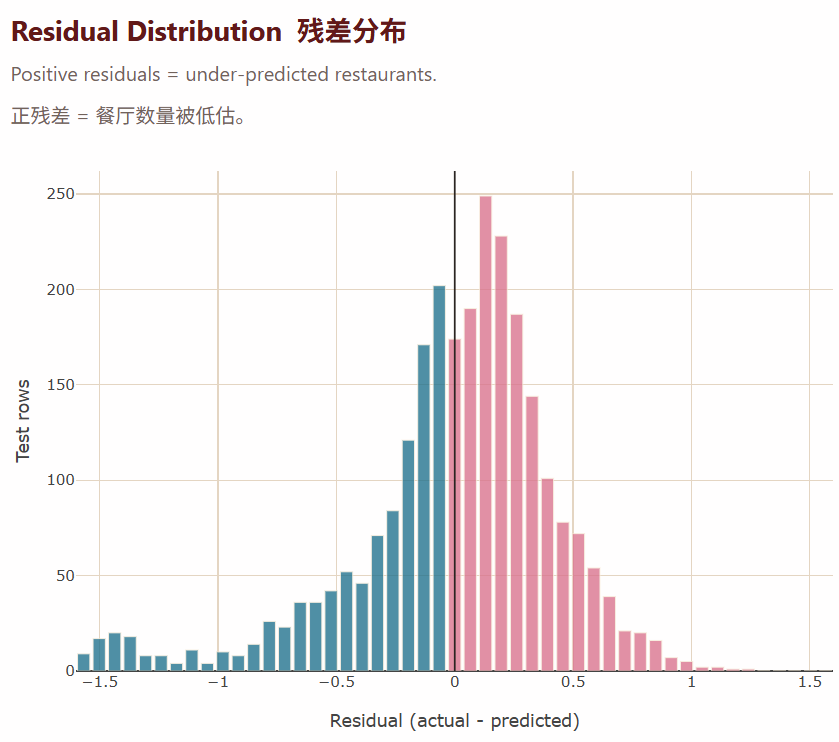
\includegraphics[width=0.95\textwidth]{figures/15_residual_analysis.png}
\caption{残差分析与分布}
\label{fig:residual}
\end{figure}

图~\ref{fig:residual} 展示了残差的直方图分布。正值残差表示模型低估，负值表示模型高估。残差分布接近正态，说明模型没有明显的系统性偏差。

\begin{figure}[H]
\centering
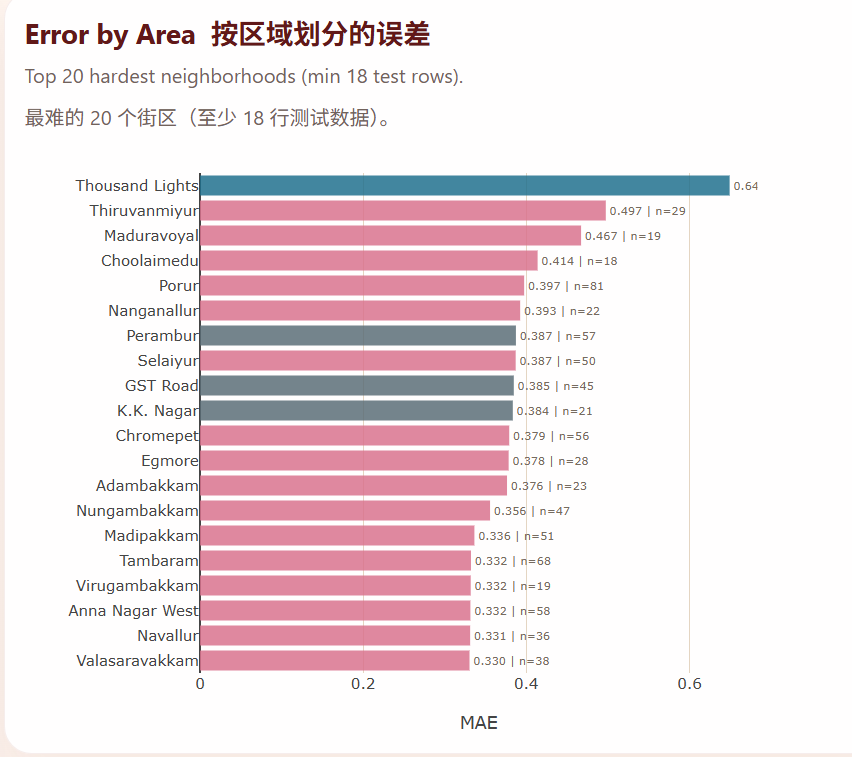
\includegraphics[width=0.95\textwidth]{figures/16_area_mae_bias.png}
\caption{按区域分解 MAE 与 Bias}
\label{fig:area_mae}
\end{figure}

图~\ref{fig:area_mae} 按区域分解预测误差，展示了不同区域的 MAE 和 Bias。这有助于识别模型在哪些区域的预测质量较差，可能暗示这些区域存在未被特征捕获的局部模式。

\begin{figure}[H]
\centering
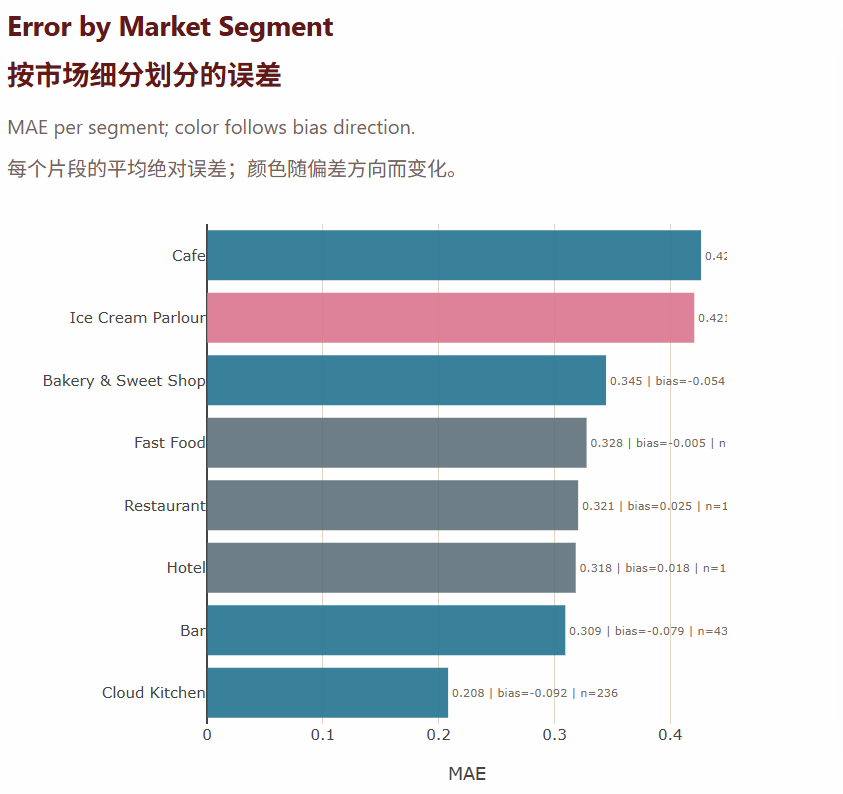
\includegraphics[width=0.95\textwidth]{figures/17_segment_mae_bias.png}
\caption{按市场细分分解 MAE 与 Bias}
\label{fig:segment_mae}
\end{figure}

图~\ref{fig:segment_mae} 按市场细分分解预测误差。不同业态的预测难度不同，这可能与各业态的评分驱动因素差异有关。

\subsubsection{特征重要性与可解释性分析}

\begin{figure}[H]
\centering
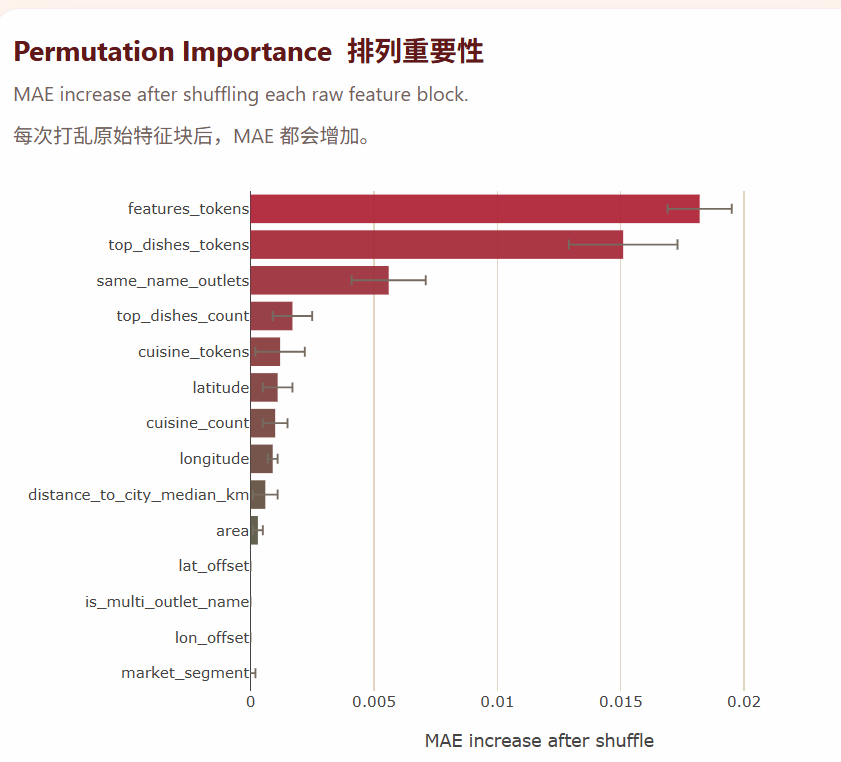
\includegraphics[width=0.95\textwidth]{figures/18_feature_importance.png}
\caption{Permutation Importance 特征重要性排名}
\label{fig:importance}
\end{figure}

图~\ref{fig:importance} 展示了置换重要性（Permutation Importance）排名。置换重要性的原理是：随机打乱某个特征的值后，观察模型性能的下降幅度，下降越多说明该特征越重要。

\begin{figure}[H]
\centering
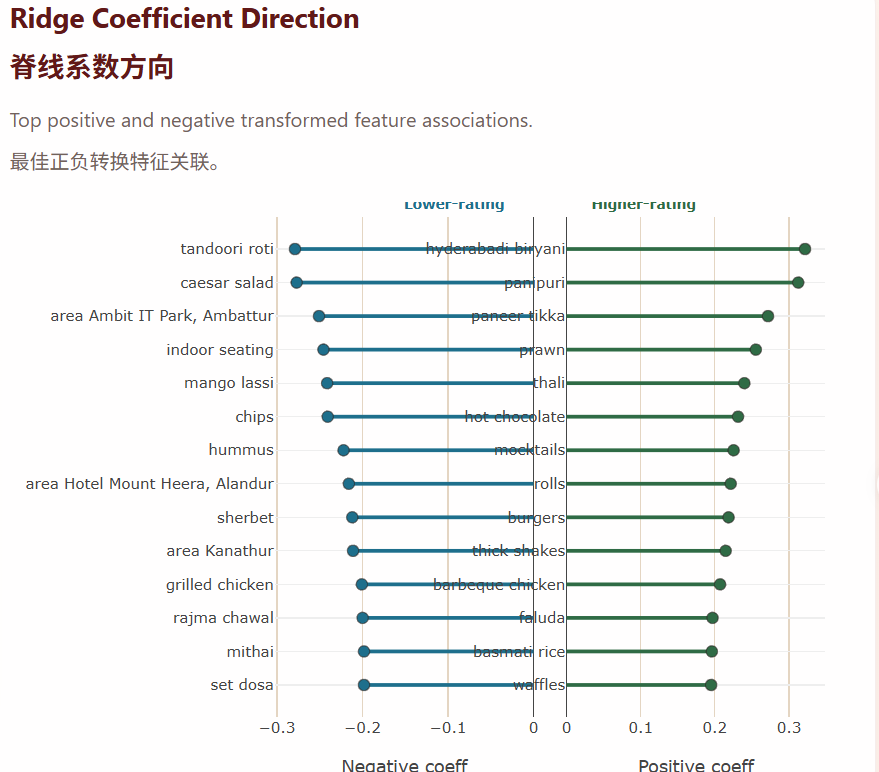
\includegraphics[width=0.95\textwidth]{figures/19_ridge_coefficients.png}
\caption{Ridge 回归系数方向图}
\label{fig:ridge_coef}
\end{figure}

图~\ref{fig:ridge_coef} 展示了 Ridge 回归的系数方向，正向系数表示该特征与评分正相关，负向系数表示负相关。结合置换重要性图，可以更全面地理解特征对评分的影响方向和强度。

综合现有预测结果，可以得出以下判断：
\begin{itemize}[leftmargin=2em]
    \item \textbf{品牌足迹}（同名门店数 same\_name\_outlets）是评分最强正向预测因子之一，说明连锁品牌的质量控制更稳定；
    \item \textbf{距离市中心越远}（distance\_to\_city\_median\_km），评分往往越低，可能与商圈成熟度和人流量有关；
    \item \textbf{招牌菜丰富度}（top\_dishes token 数）对评分有正向贡献，菜品丰富的餐厅往往评分更高；
    \item \textbf{Cloud Kitchen / Dine-out} 的预测评分最高，与前面的市场细分分析结论一致。
\end{itemize}

% ==================== 第五章 总结 ====================
\section{总结}

\subsection{研究成果与主要发现}

本研究围绕 Chennai 餐饮市场的探索性数据分析与可视化问题，完成了从数据预处理、统计分析、空间分析、图表设计到机器学习预测的完整流程，取得了以下主要成果：

\begin{enumerate}[leftmargin=2em]
    \item 构建了面向真实餐饮平台数据的分析流程，完成了字段规范化、多值文本展开、衍生特征构造和多视角聚合分析。原始数据经过预处理后，从 11,848 行的宽表展开为合计超过 138,000 行的长格式数据，为多维度分析提供了数据基础。

    \item 通过多种静态与交互式可视化手段（涵盖柱状图、脊线图、热力图、箱线图、堆叠图、气泡图、核密度热力图、四象限矩阵图、词云图等 10 余种图表类型），系统展示了市场细分差异、区域供给分布、菜系与菜品结构以及服务特征关系。

    \item 识别出 Chennai 餐饮市场的几类核心规律：
    \begin{itemize}[leftmargin=1.5em]
        \item Dine-out 主导规模（5,292 家），Cloud Kitchen 平均评分最高（3.68）；
        \item 空间分布存在明显异质性，T. Nagar / Anna Nagar 为核心优质区；
        \item 本地菜（Biryani、Dosa、Idli、Filter Coffee）与高频服务特征（Home Delivery、Indoor Seating）能有效刻画消费文化；
        \item 品牌足迹与地理位置对评分预测具有重要作用。
    \end{itemize}

    \item 将机器学习预测模块纳入 EDA 体系中，实现了"描述市场 $\rightarrow$ 解释市场 $\rightarrow$ 预测市场"的分析闭环。通过 Permutation Importance 和偏依赖分析，从数据驱动的角度验证了品牌效应、地理位置和菜品丰富度对评分的影响。
\end{enumerate}

\subsection{课程知识点运用效果分析}

从课程知识点角度看，本项目较全面地体现了探索性数据分析与可视化技术的综合运用效果：

\begin{enumerate}[leftmargin=2em]
    \item \textbf{数据处理层面}：完成了缺失值检查、字段统一、长宽表变换和特征工程，说明项目能够针对原始数据中的结构问题进行规范化处理。特别是多值文本展开（cuisine/features/top\_dishes）和衍生特征构造（rating\_band、品牌足迹、空间偏移）体现了从原始字段到分析变量的转化思路。

    \item \textbf{分析层面}：综合运用了描述统计、分组聚合、分布分析、空间分析和模型解释方法，体现了从"看数据"到"懂数据"的递进过程。脊线图、四象限矩阵和核密度热力图等方法的运用，展示了对多种 EDA 手段的灵活组合能力。

    \item \textbf{可视化设计层面}：图表类型与变量特性匹配度较高，且兼顾了美观性与信息表达效率。统一的暖色美食主题配色、清晰的标题和标注、辅助函数的使用，体现了可视化设计的规范性和一致性。

    \item \textbf{可视分析层面}：将静态分析与交互式探索相结合，通过 Flask + Plotly/ECharts 实现了可交互的分析界面，体现了可视分析"人机结合"的核心理念。
\end{enumerate}

整体而言，项目符合课程"避免单纯技术堆砌、强调数据洞察"的目标导向。

\subsection{不足与局限性}

尽管本研究完成了较完整的分析流程，但仍存在以下局限：

\begin{itemize}[leftmargin=2em]
    \item \textbf{数据时效性局限}：平台评分和门店状态会随时间变化，当前数据仅能反映采集时点的市场状态，无法捕捉动态变化趋势；

    \item \textbf{特征维度有限}：缺少价格区间、评论量、图像信息、营业时间、用户画像等更细粒度变量，限制了分析深度和预测精度。例如，评分可能与价格区间和评论量高度相关，但这些变量在当前数据集中不可用；

    \item \textbf{空间表达仍较粗粒度}：当前主要基于区域均值和经纬度密度做分析，尚未引入道路网络、商圈边界、人口密度和 POI（兴趣点）等外部空间信息，空间分析的精度和解释力还有提升空间；

    \item \textbf{课程报告形式限制}：纸质报告中只能展示静态图，无法完整体现项目交互式页面的探索优势。交互式界面中的缩放、筛选和悬停提示等动态功能在 PDF 中无法复现。
\end{itemize}

\subsection{后续优化方向}

基于上述局限，未来可从以下方向继续优化：

\begin{enumerate}[leftmargin=2em]
    \item 引入评论数、价格等级、图像数量、营业时间等扩展特征，增强多维分析能力和预测精度；
    \item 增加时序分析模块，研究评分与市场供给的动态变化趋势，识别增长区域和衰退区域；
    \item 将区域分析扩展为更精细的空间建模，如结合 POI、路网或 DBSCAN 聚类方法进行商圈识别；
    \item 在推荐系统方向上，结合用户偏好、菜系兴趣与位置约束，构建个性化餐厅推荐方案；
    \item 将当前静态图表进一步组织成交互式数据故事（Data Story），提高可视分析的探索效率和表达层次；
    \item 引入自然语言处理（NLP）技术对用户评论进行情感分析，挖掘评分背后的具体原因。
\end{enumerate}

% ==================== 参考文献 ====================
\newpage
\begin{thebibliography}{99}

\bibitem{tukey}
J. W. Tukey, \emph{Exploratory Data Analysis}. Reading, MA, USA: Addison-Wesley, 1977.

\bibitem{heer}
J. Heer, M. Bostock, and V. Ogievetsky, ``A tour through the visualization zoo,'' \emph{Communications of the ACM}, vol. 53, no. 6, pp. 59--67, 2010.

\bibitem{ward}
M. Ward, G. Grinstein, and D. Keim, \emph{Interactive Data Visualization: Foundations, Techniques, and Applications}. Natick, MA, USA: A K Peters, 2015.

\bibitem{wilkinson}
L. Wilkinson, \emph{The Grammar of Graphics}, 2nd ed. New York, NY, USA: Springer, 2005.

\bibitem{tufte}
E. R. Tufte, \emph{The Visual Display of Quantitative Information}, 2nd ed. Cheshire, CT, USA: Graphics Press, 2001.

\bibitem{cleveland}
W. S. Cleveland and R. McGill, ``Graphical perception: Theory, experimentation, and application to the development of graphical methods,'' \emph{Journal of the American Statistical Association}, vol. 79, no. 387, pp. 531--554, 1984.

\bibitem{scikit}
F. Pedregosa \emph{et al.}, ``Scikit-learn: Machine learning in Python,'' \emph{Journal of Machine Learning Research}, vol. 12, pp. 2825--2830, 2011.

\bibitem{plotly}
Plotly Technologies Inc., ``Collaborative data science,'' 2015. [Online]. Available: \url{https://plotly.com/}

\bibitem{zomato}
Devvraj, ``Chennai restaurant dataset,'' Kaggle, accessed 2026. [Online]. Available: \url{https://www.kaggle.com/datasets/devvraj/chennai-restaurant-dataset}

\bibitem{mckinney}
W. McKinney, ``pandas: a foundational Python library for data analysis and statistics,'' \emph{Python for High Performance and Scientific Computing}, 2011.

\bibitem{hastie}
T. Hastie, R. Tibshirani, and J. Friedman, \emph{The Elements of Statistical Learning}, 2nd ed. New York, NY, USA: Springer, 2009.

\end{thebibliography}

\end{document}
